\chapter{Metodologia}
\label{cap:metodologia}

Nesse capítulo serão abordados os métodos utilizados para encontrar e selecionar juízes \textit{online}, os métodos de desenvolvimento do GOJ, os critérios para seleção de juízes \textit{online}, os métodos de contagem de seus problemas, a arquitetura geral do GOJ, a arquitetura e tecnologias utilizadas em cada um dos módulos do sistema.

\section{Produtos relacionados}

Para o desenvolvimento do GOJ, uma das etapas foi identificar os principais juízes online, para observação das funcionalidades e características de cada um deles. Para isso foi realizada uma busca por juízes online e uma seleção de alguns desses juízes. Depois, foi feito um levantamento de funcionalidades e do número de problemas de cada um.

Nessa seção serão descritos os métodos para a identificação dos principais juízes onlines existentes, os métodos para levantamento do número de questões e das funcionalidades em cada um deles, além disso, serão apresentados os critérios de seleção dos juízes.

\subsection{Identificação dos principais juízes online exisitentes}
\label{subsec:selecao_juizes}

Conforme definido na Seção \ref{sec:juizesOnline}, um juiz \textit{online} é um site ou página que armazena problemas e possibilita ao usuário enviar suas soluções para o problema, para que estas soluções sejam avaliadas e que o usuário receba um veredito. A identificação dos principais juízes \textit{online} existentes foi feita com base em pesquisas de termos específicos no \textit{Google}\footnote{\url{https://www.google.com/}}, mecanismo de pesquisas \textit{online}. Para a seleção de resultados foram considerados apenas os sites que se encaixaram na definição de juiz \textit{online} citada. Apenas as duas primeiras páginas retornadas na pesquisa foram consideradas para cada uma das buscas. Os resultados estão enumerados em ordem de relevância, determinada pelo mecanismo de pesquisa do Google, que lista os resultados mais relevantes primeiro, ou seja, em ordem de aparição. Vale ressaltar que os resultados das buscas listam páginas de anúncios, porém, estes anúncios foram desconsiderados.

A primeira busca realizada foi com o termo ``\textit{online judge}'', e obteve os seguintes resultados: ``\textit{online judge}'': o Online Judge\footnote{\url{https://www.onlinejudge.org/}}, conhecido anteriormente como \textit{UVa};
o Beecrowd\footnote{\url{https://www.beecrowd.com.br}}, antigo URI,
o Sphere Online Judge (SPOJ)\footnote{\url{https://www.spoj.com/}}, e o PKU JudgeOnline\footnote{\url{http://poj.org/}}, o juiz \textit{online} da Universidade de Pequim.

A segunda busca foi realizada com o termo ``\textit{online programming contests}'' e os resultados foram:

\begin{enumerate}
    \item CodeChef
    \item Google's Coding Competitions
    \item Beecrowd
    \item Sphere Online Judge (SPOJ)
    \item Hackerearth
\end{enumerate}

O novo termo foi utilizado com o propósito de identificar sites que, além de serem juízes \textit{online}, possuem competições de programação. Como consequência, o resultado listou juízes diferentes daqueles relacionados na busca anterior. São eles: CodeChef\footnote{\url{https://www.codechef.com/}}, um juiz \textit{online} que possui alguns diferenciais como competições e o armazenamento de questões das competições passadas para práticas posteriores; Goolge's Coding Competitions\footnote{\url{https://codingcompetitions.withgoogle.com/}}, site onde estão reunidos \textit{links} para competições do Google como Kick Start\footnote{\url{https://codingcompetitions.withgoogle.com/kickstart/about/}}, Hash Code\footnote{\url{https://codingcompetitions.withgoogle.com/hashcode/about/}} e CodeJam\footnote{\url{https://codingcompetitions.withgoogle.com/codejam/about/}}; e por fim, o Hackerearth\footnote{\url{https://www.hackerearth.com/}}, site muito usado para prática de entrevistas técnicas de programação e que oferece um serviço de entrevista técnica para empresas, onde permite que os candidatos realizem entrevistas técnicas na plataforma, com o acompanhamento de um entrevistador.

O terceiro termo pesquisado foi ``\textit{programming competitions and contests}'', e os resultados foram:

\begin{enumerate}
    \item Google's Coding Competitions
    \item CodeChef
    \item Codeforces
    \item Hackerearth
\end{enumerate}

Este terceiro termo tinha como objetivo ressaltar sites de competição e o único site novo que apareceu foi o Codeforces\footnote{\url{https://codeforces.com/}}, um site voltado para competições de programação que possui um vasto número de problemas para práticas posteriores. Assim, se tornam diferencias do site as competições e as questões de competições passadas para práticas posteriores.

A quarta busca foi utilizando o termo ``juiz \textit{online} programação'', e os resultados foram:

\begin{enumerate}
    \item Beecrowd
    \item Neps Academy 
    \item CodeBench
\end{enumerate}

O quarto termo foi construído propositalmente usando duas palavras da língua portuguesa, para deste modo tentar encontrar juízes \textit{online} com questões em português, ou que possuem o português do Brasil como um dos idiomas dos textos. Esta quarta busca obteve dois novos resultados: Neps Academy\footnote{\url{https://neps.academy/}}, um site voltado para o ensino de programação, que possui como diferenciais aulas, competições e o armazenamento das questões de competições para práticas posteriores; e o CodeBench\footnote{\url{https://codebench.icomp.ufam.edu.br/}}, site voltado para ensino, com criação de turma e inscrição de alunos. 

Também foram pesquisados os termos ``programação'' e``\textit{contests} de programação'', porém não foram encontrados novos resultados.

\subsection{Levantamento do número de problemas}
\label{subsec:levantamento_numero_de_problemas}

Em cada um dos juízes selecionados na Subseção \ref{subsec:selecao_juizes} foi realizado um levantamento do número total de problemas disponíveis para seus usuários. Para isso, distintas abordagens foram escolhidas conforme as diferentes características de cada juiz \textit{online}. Nessa subseção serão apresentadas as abordagens e estratégias utilizadas para esta contagem de problemas.

Para o levantamento dos problemas da plataforma Online Judge foi acessada a aba \textit{Browse Problems}\footnote{\url{https://onlinejudge.org/index.php?option=com\_onlinejudge\&Itemid=8}}, conforme mostra a Figura \ref{fig:online_judge_1}. Em cada uma das categorias foi contado o número de problemas presentes (veja a Figura \ref{fig:online_judge_2}). Esta contagem foi realizada por um \textit{script} em linguagem de programação Python, disponível no Apêndice \ref{appendix:script_oj}, com a estratégia de localizar o padrão em \textit{links} de categorias e \textit{links} de problemas. O primeiro padrão observado é que as pastas ficam em uma tabela; ao localizar a tabela pelo HTML da página é possível encurtar a busca pelos links. O segundo padrão que vale ressaltar é que os problemas possuem o trecho ``\texttt{page=show\_problem}'' na (URL), e isso diferencia um \textit{link} de outra pasta de um \textit{link} de problema.

\begin{figure}
    \centering
    \caption{Online Judge — Browse Problems}
    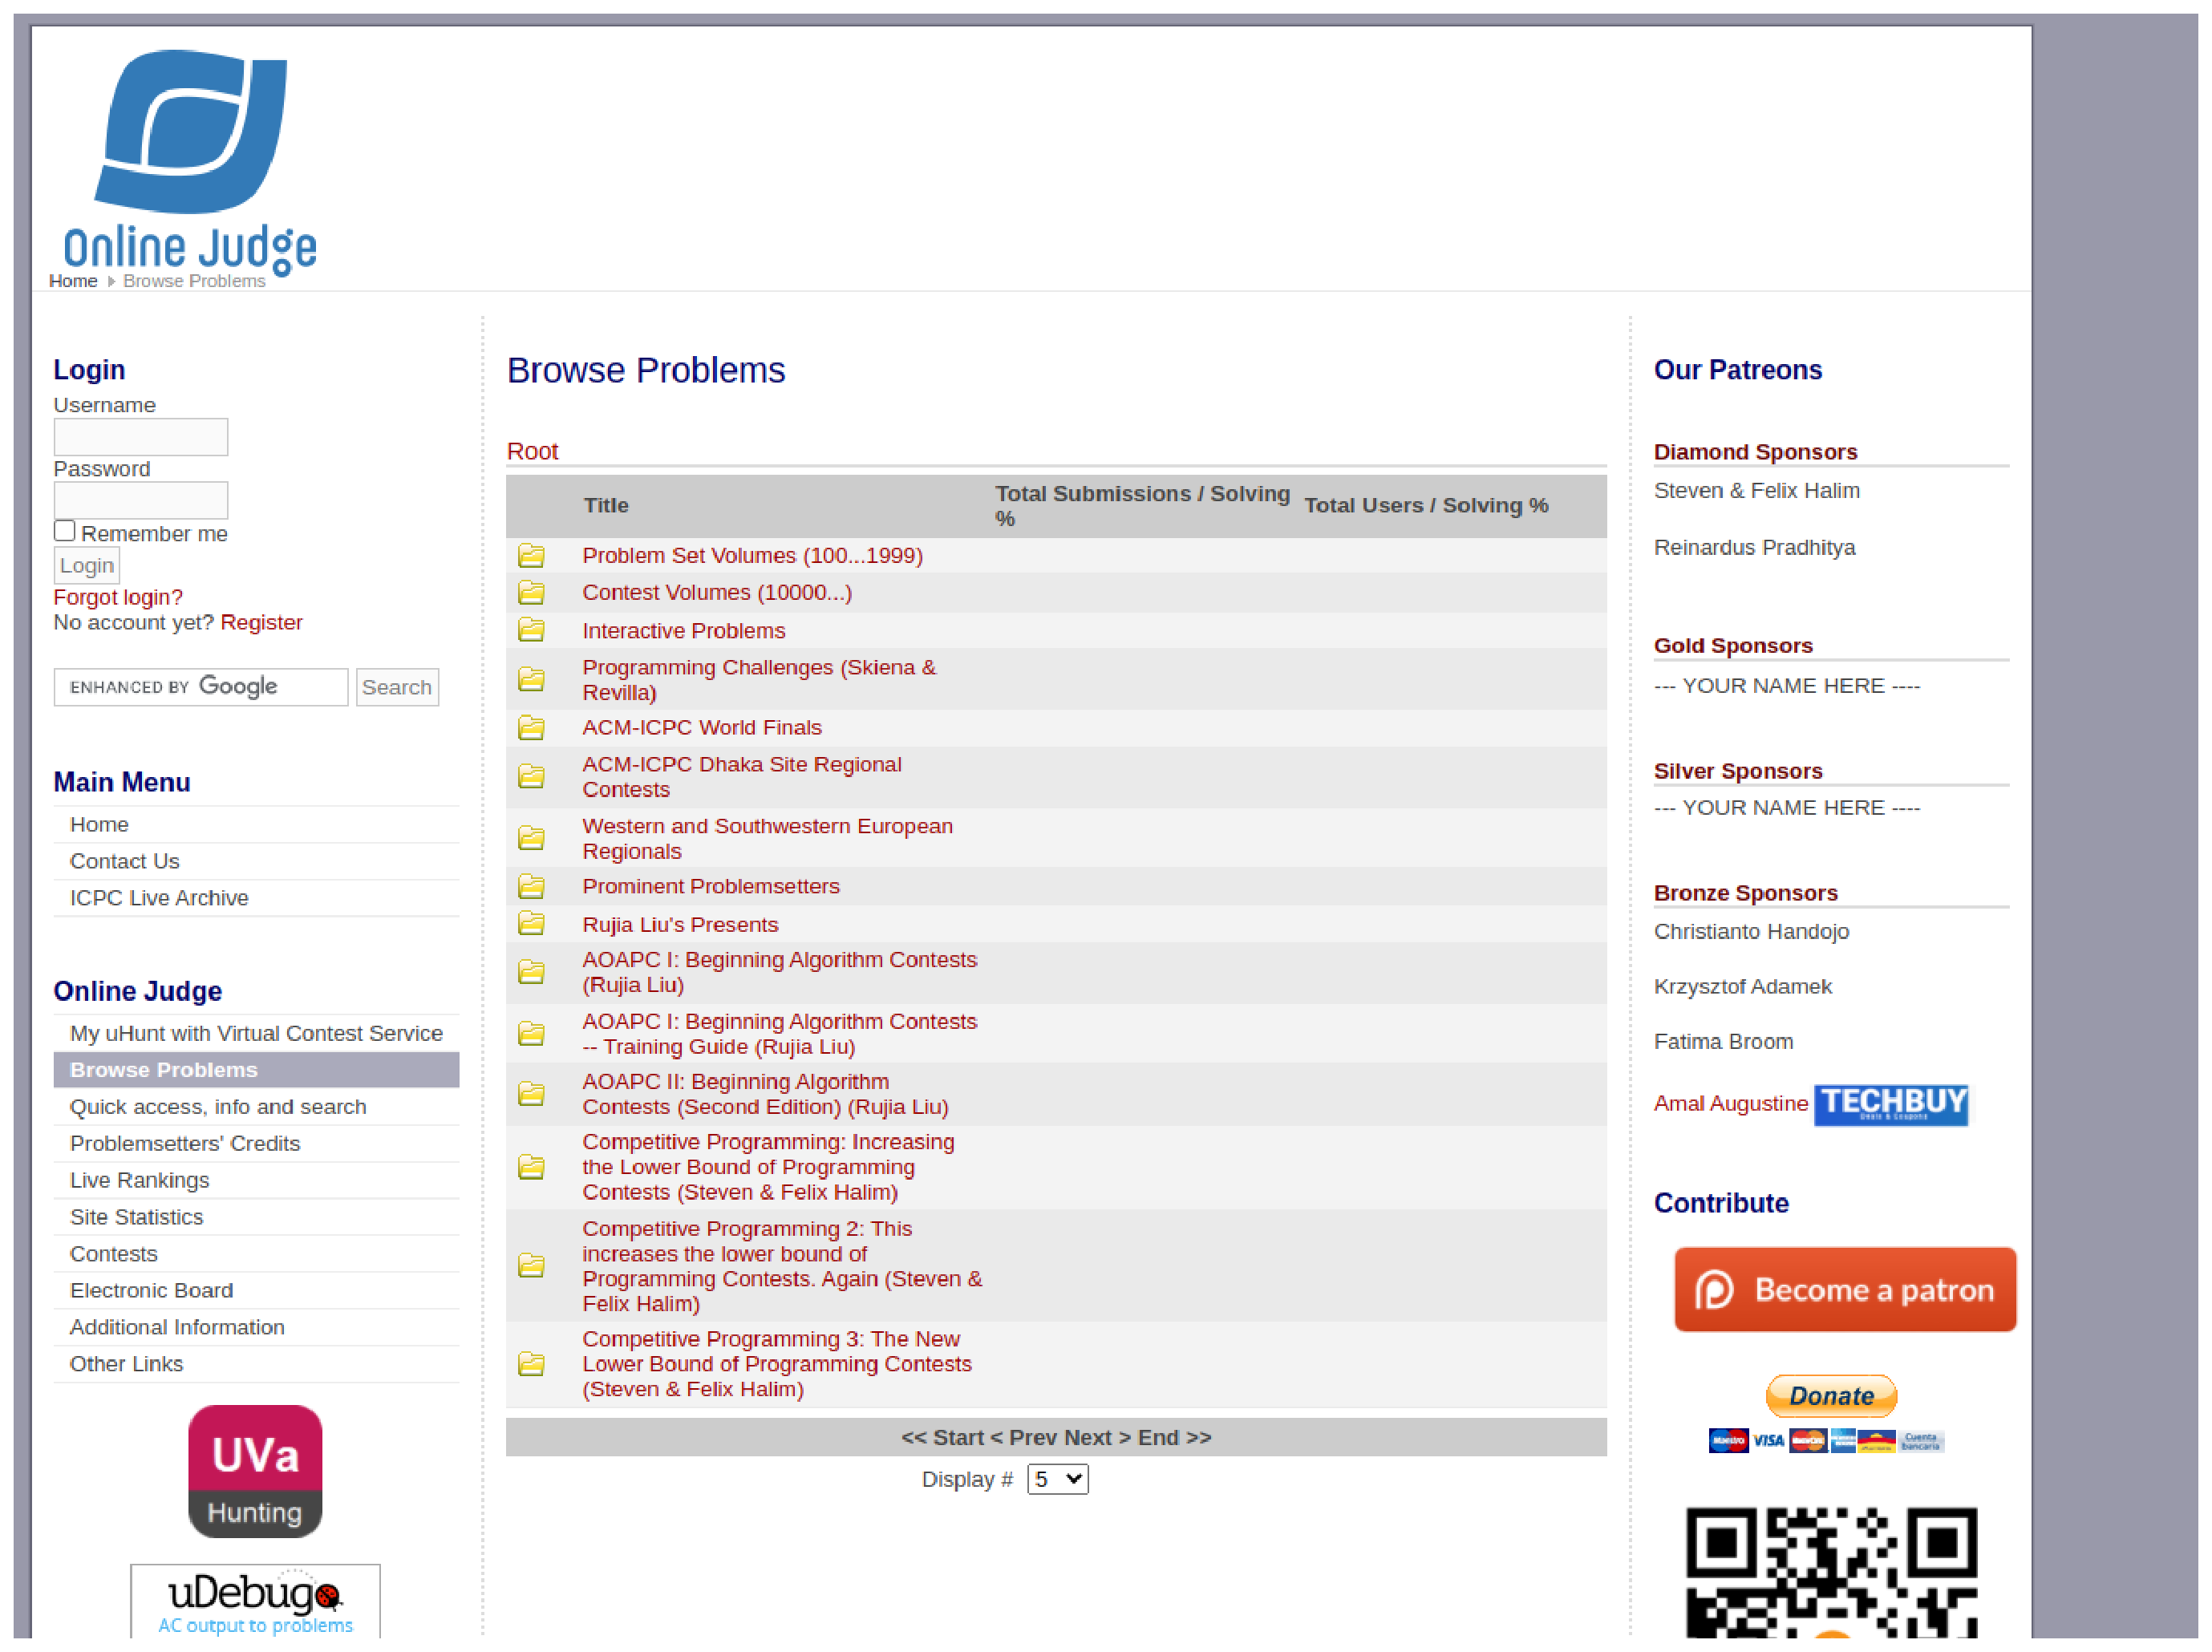
\includegraphics[keepaspectratio=true,scale=0.32]{figuras/online_judge_1.eps}
    \label{fig:online_judge_1}
    
    \medskip
    Fonte: Online Judge (\url{https://onlinejudge.org})
    \medskip
    
\end{figure}

\begin{figure}
    \centering
    \caption{Online Judge — Browse Problems (Detalhes)}
    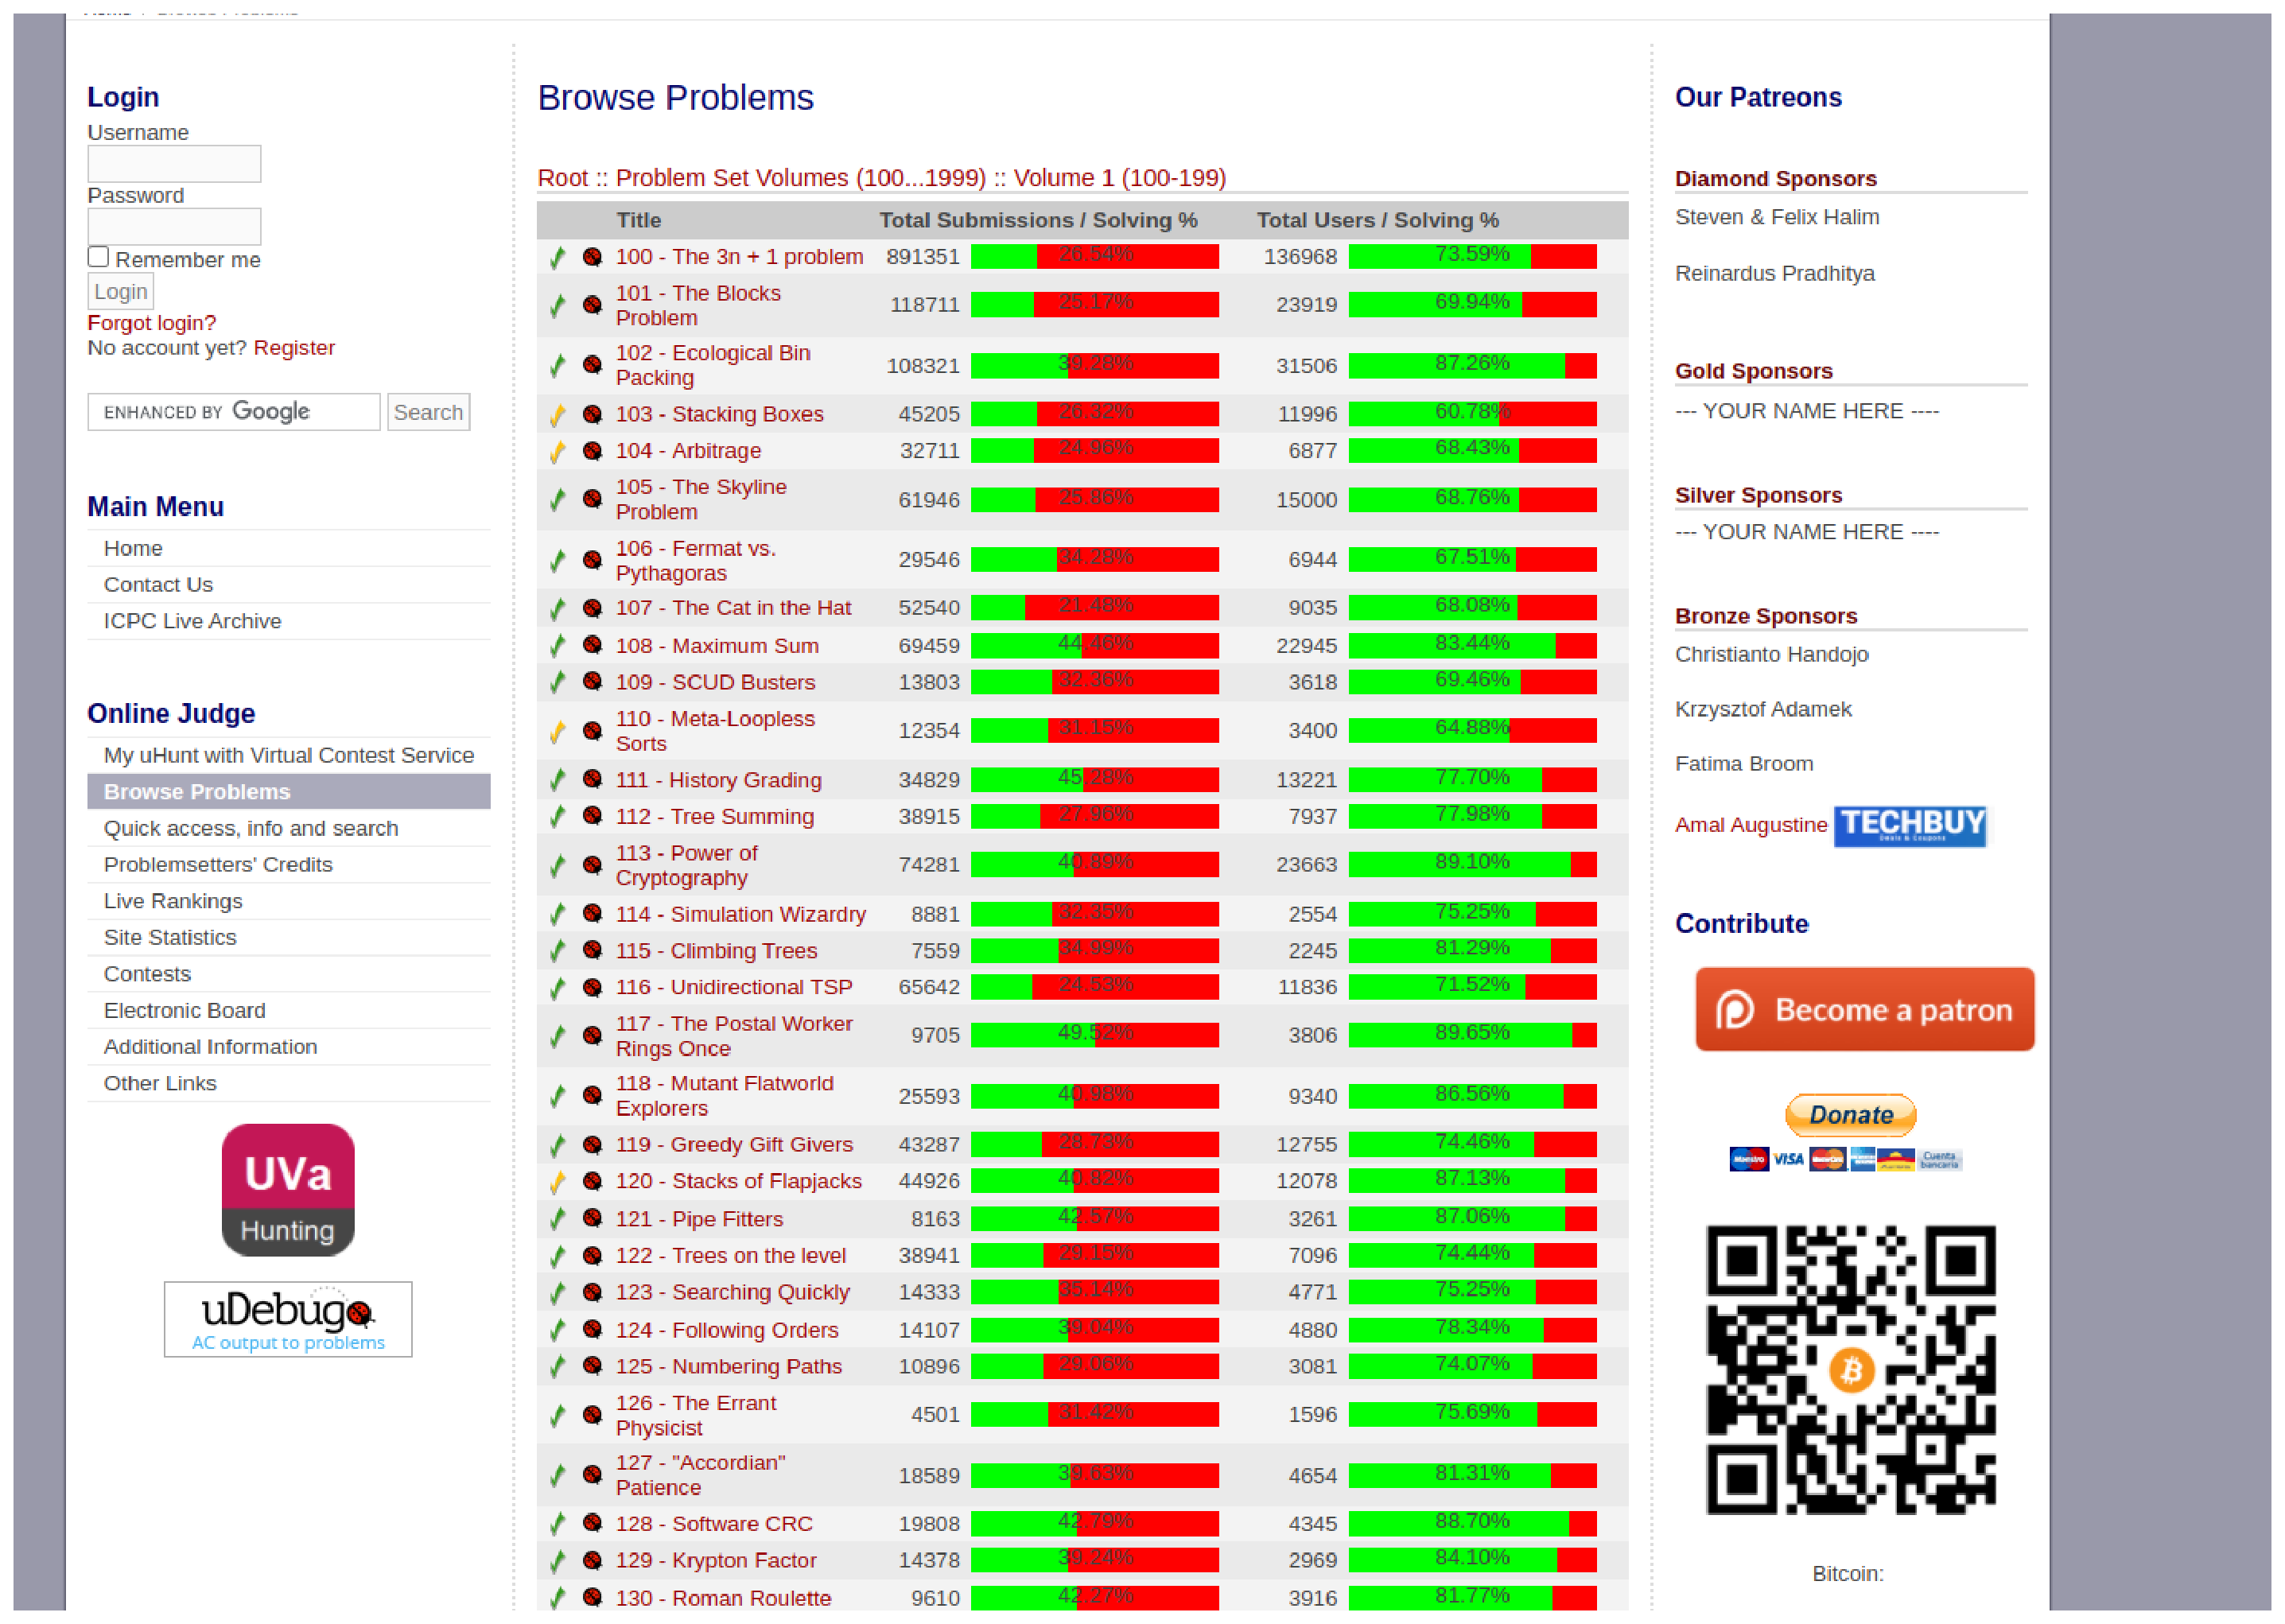
\includegraphics[keepaspectratio=true,scale=0.32]{figuras/online_judge_2.eps}
    \label{fig:online_judge_2}
    
    \medskip
    Fonte: Online Judge (\url{https://onlinejudge.org})
    \medskip
    
\end{figure}

No site Beecrowd foi preciso acessar a \textit{URL} de categorias\footnote{\url{https://www.beecrowd.com.br/judge/pt/categories}}, onde o número de problemas é exibido na categoria ``Listar todos'', conforme apresentado na Figura \ref{fig:beecrowd_1}.

\begin{figure}
    \centering
    \caption{Beecrowd — Total de problemas}
    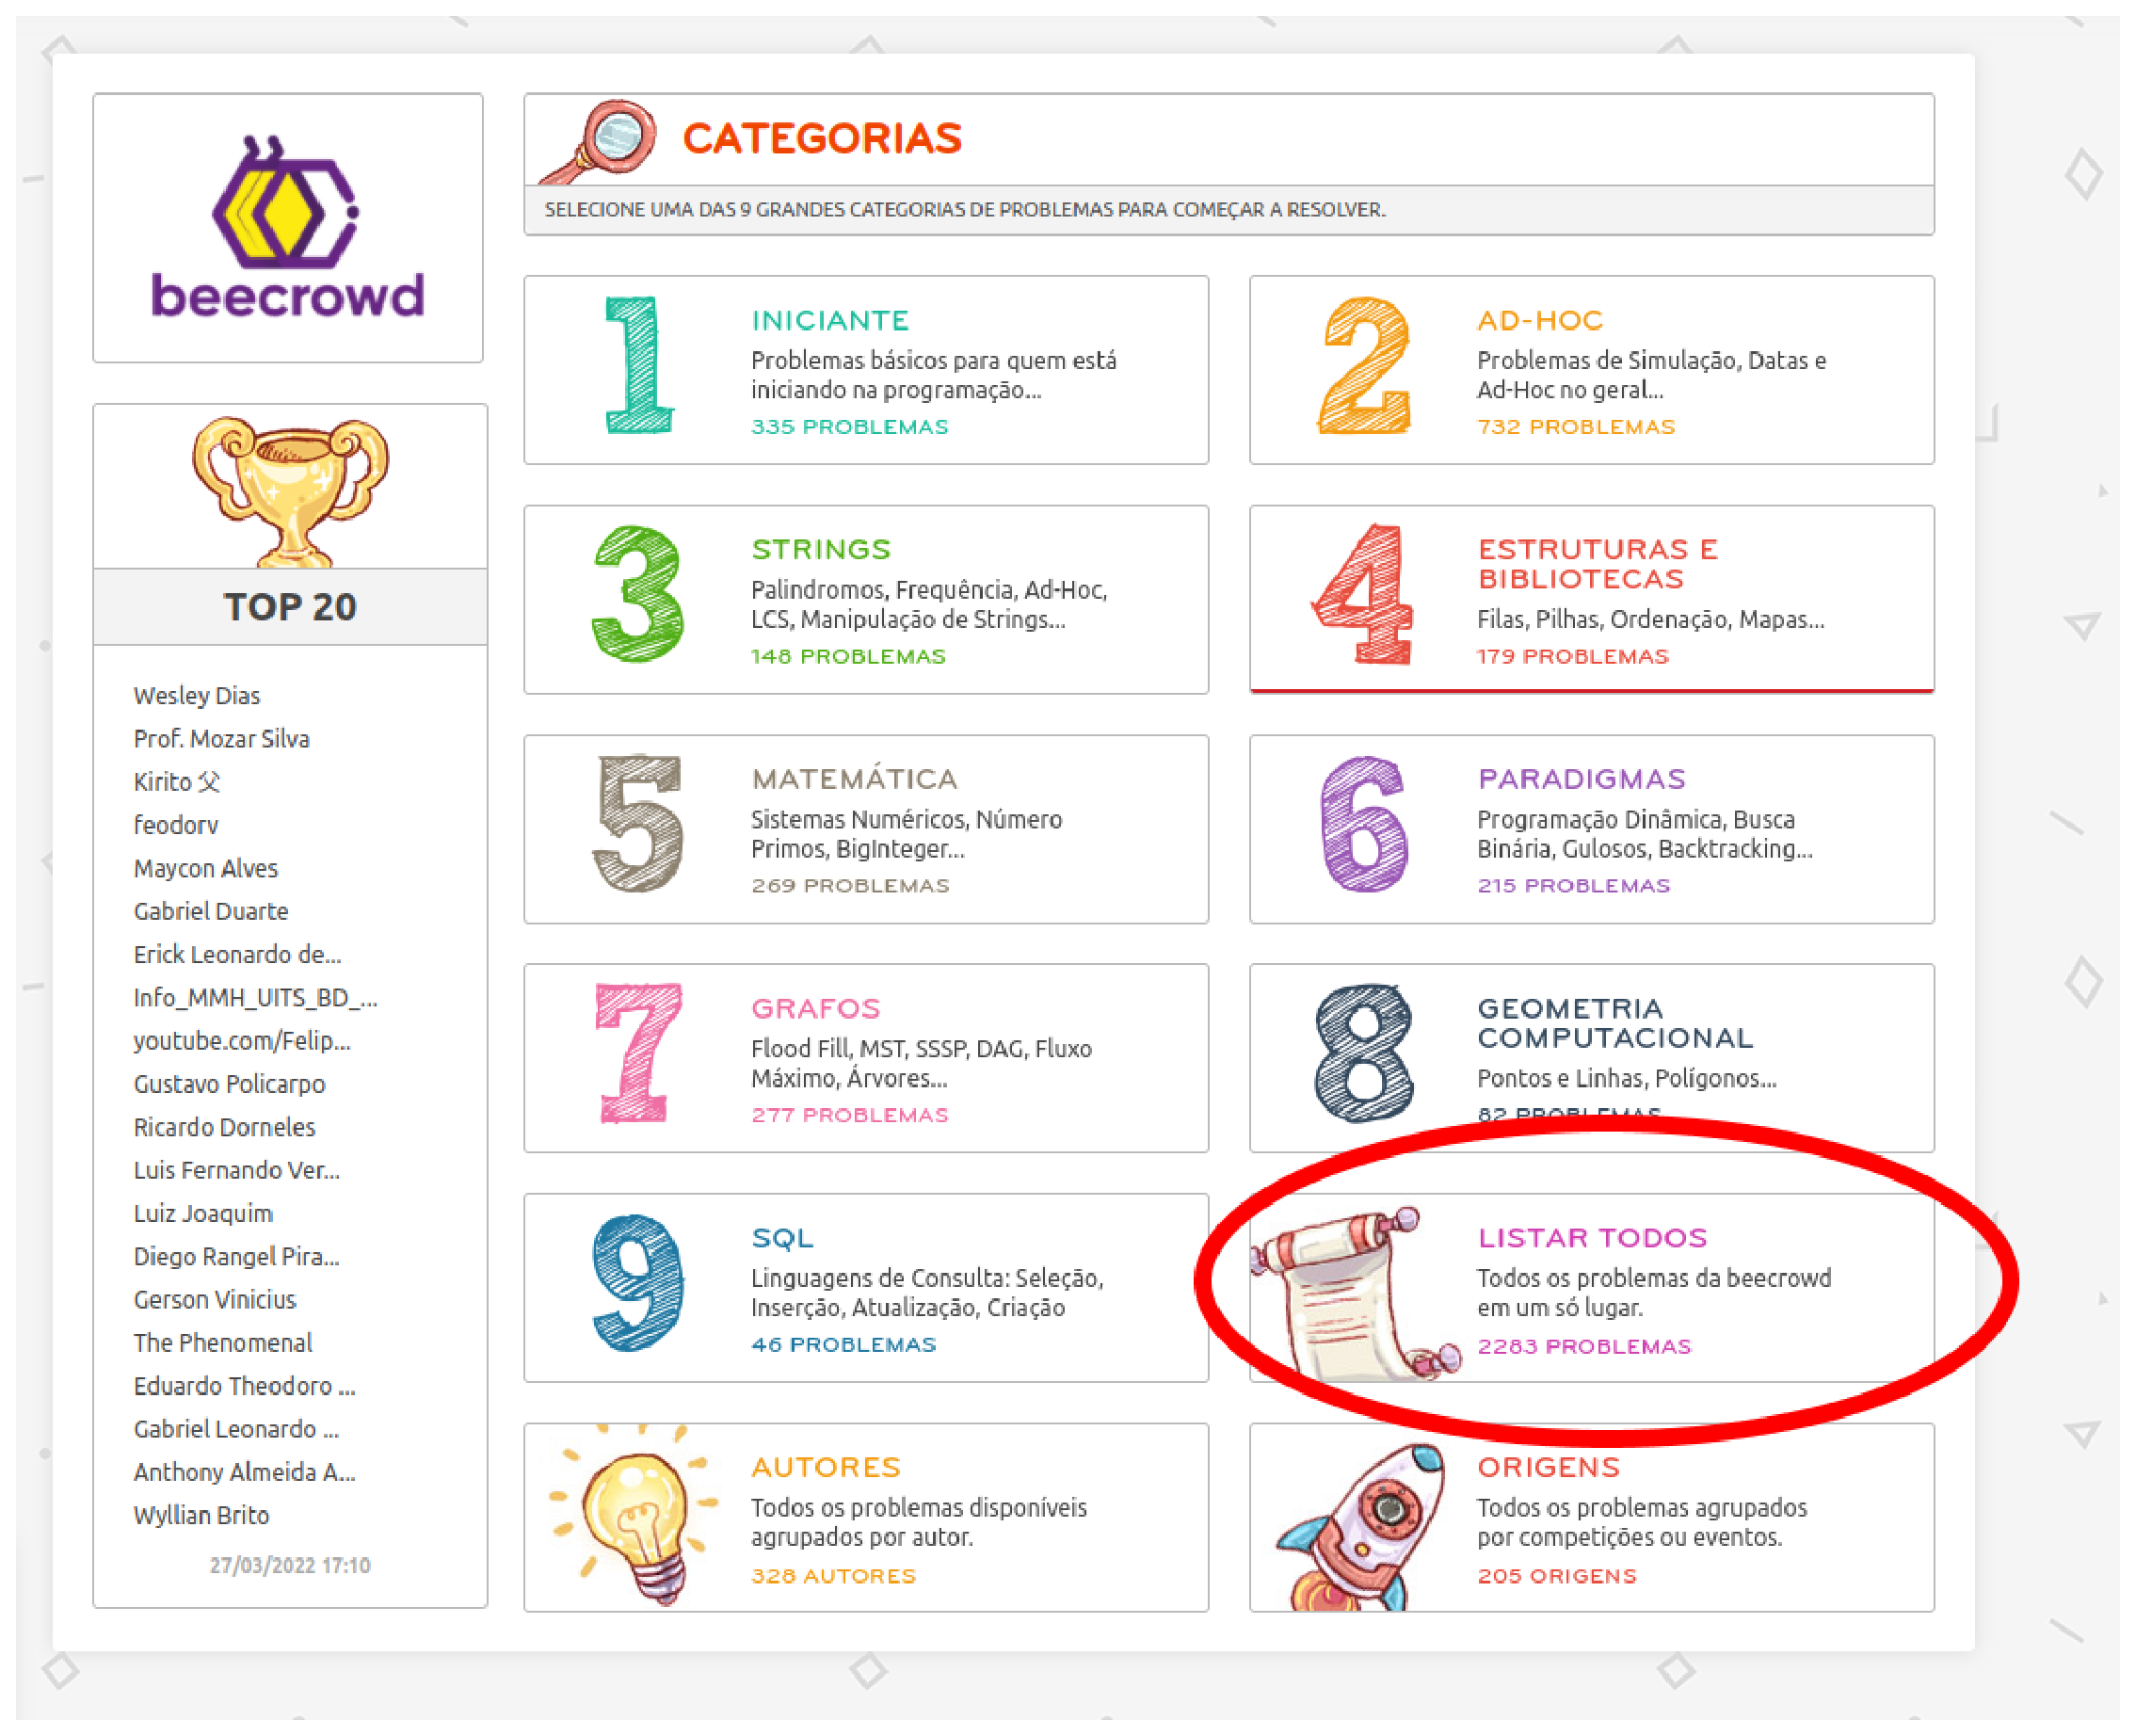
\includegraphics[keepaspectratio=true,scale=0.4]{figuras/beecrowd_1.eps}
    \label{fig:beecrowd_1}
    
    \medskip
    Fonte: Beecrowd (\url{https://www.beecrowd.com.br})
    \medskip
\end{figure}

No Codeforces foi utilizada a \textit{API} pública do site\footnote{\url{https://codeforces.com/apiHelp}}, que possui recursos para acessar as informações da plataforma; a \textit{API} é acessada via protocolo \textit{HTTP} e possui \textit{endpoints} públicos e privados. Um dos \textit{endpoints} públicos permite a visualização das informações dos problemas, retornando todos os problemas quando nenhum filtro é informado. Para recuperação do número total de problemas foi utilizado um \textit{script} em linguagem \textit{bash}, disponível no Apêndice \ref{appendix:script_cf}.

Para o levantamento do total de problemas do site CodeChef foi acessada a página de problemas, e dentro dela, foi utilizado o filtro \textit{``All Levels''}, que revelou os problemas de todos os níveis, como apresentado na Figura \ref{fig:code_chef_1}. Com isso, foi possível observar o número de problemas mais abaixo, conforme mostra a Figura \ref{fig:code_chef_2}.

\begin{figure}
    \centering
    \caption{Code Chef — Filtro de problemas}
    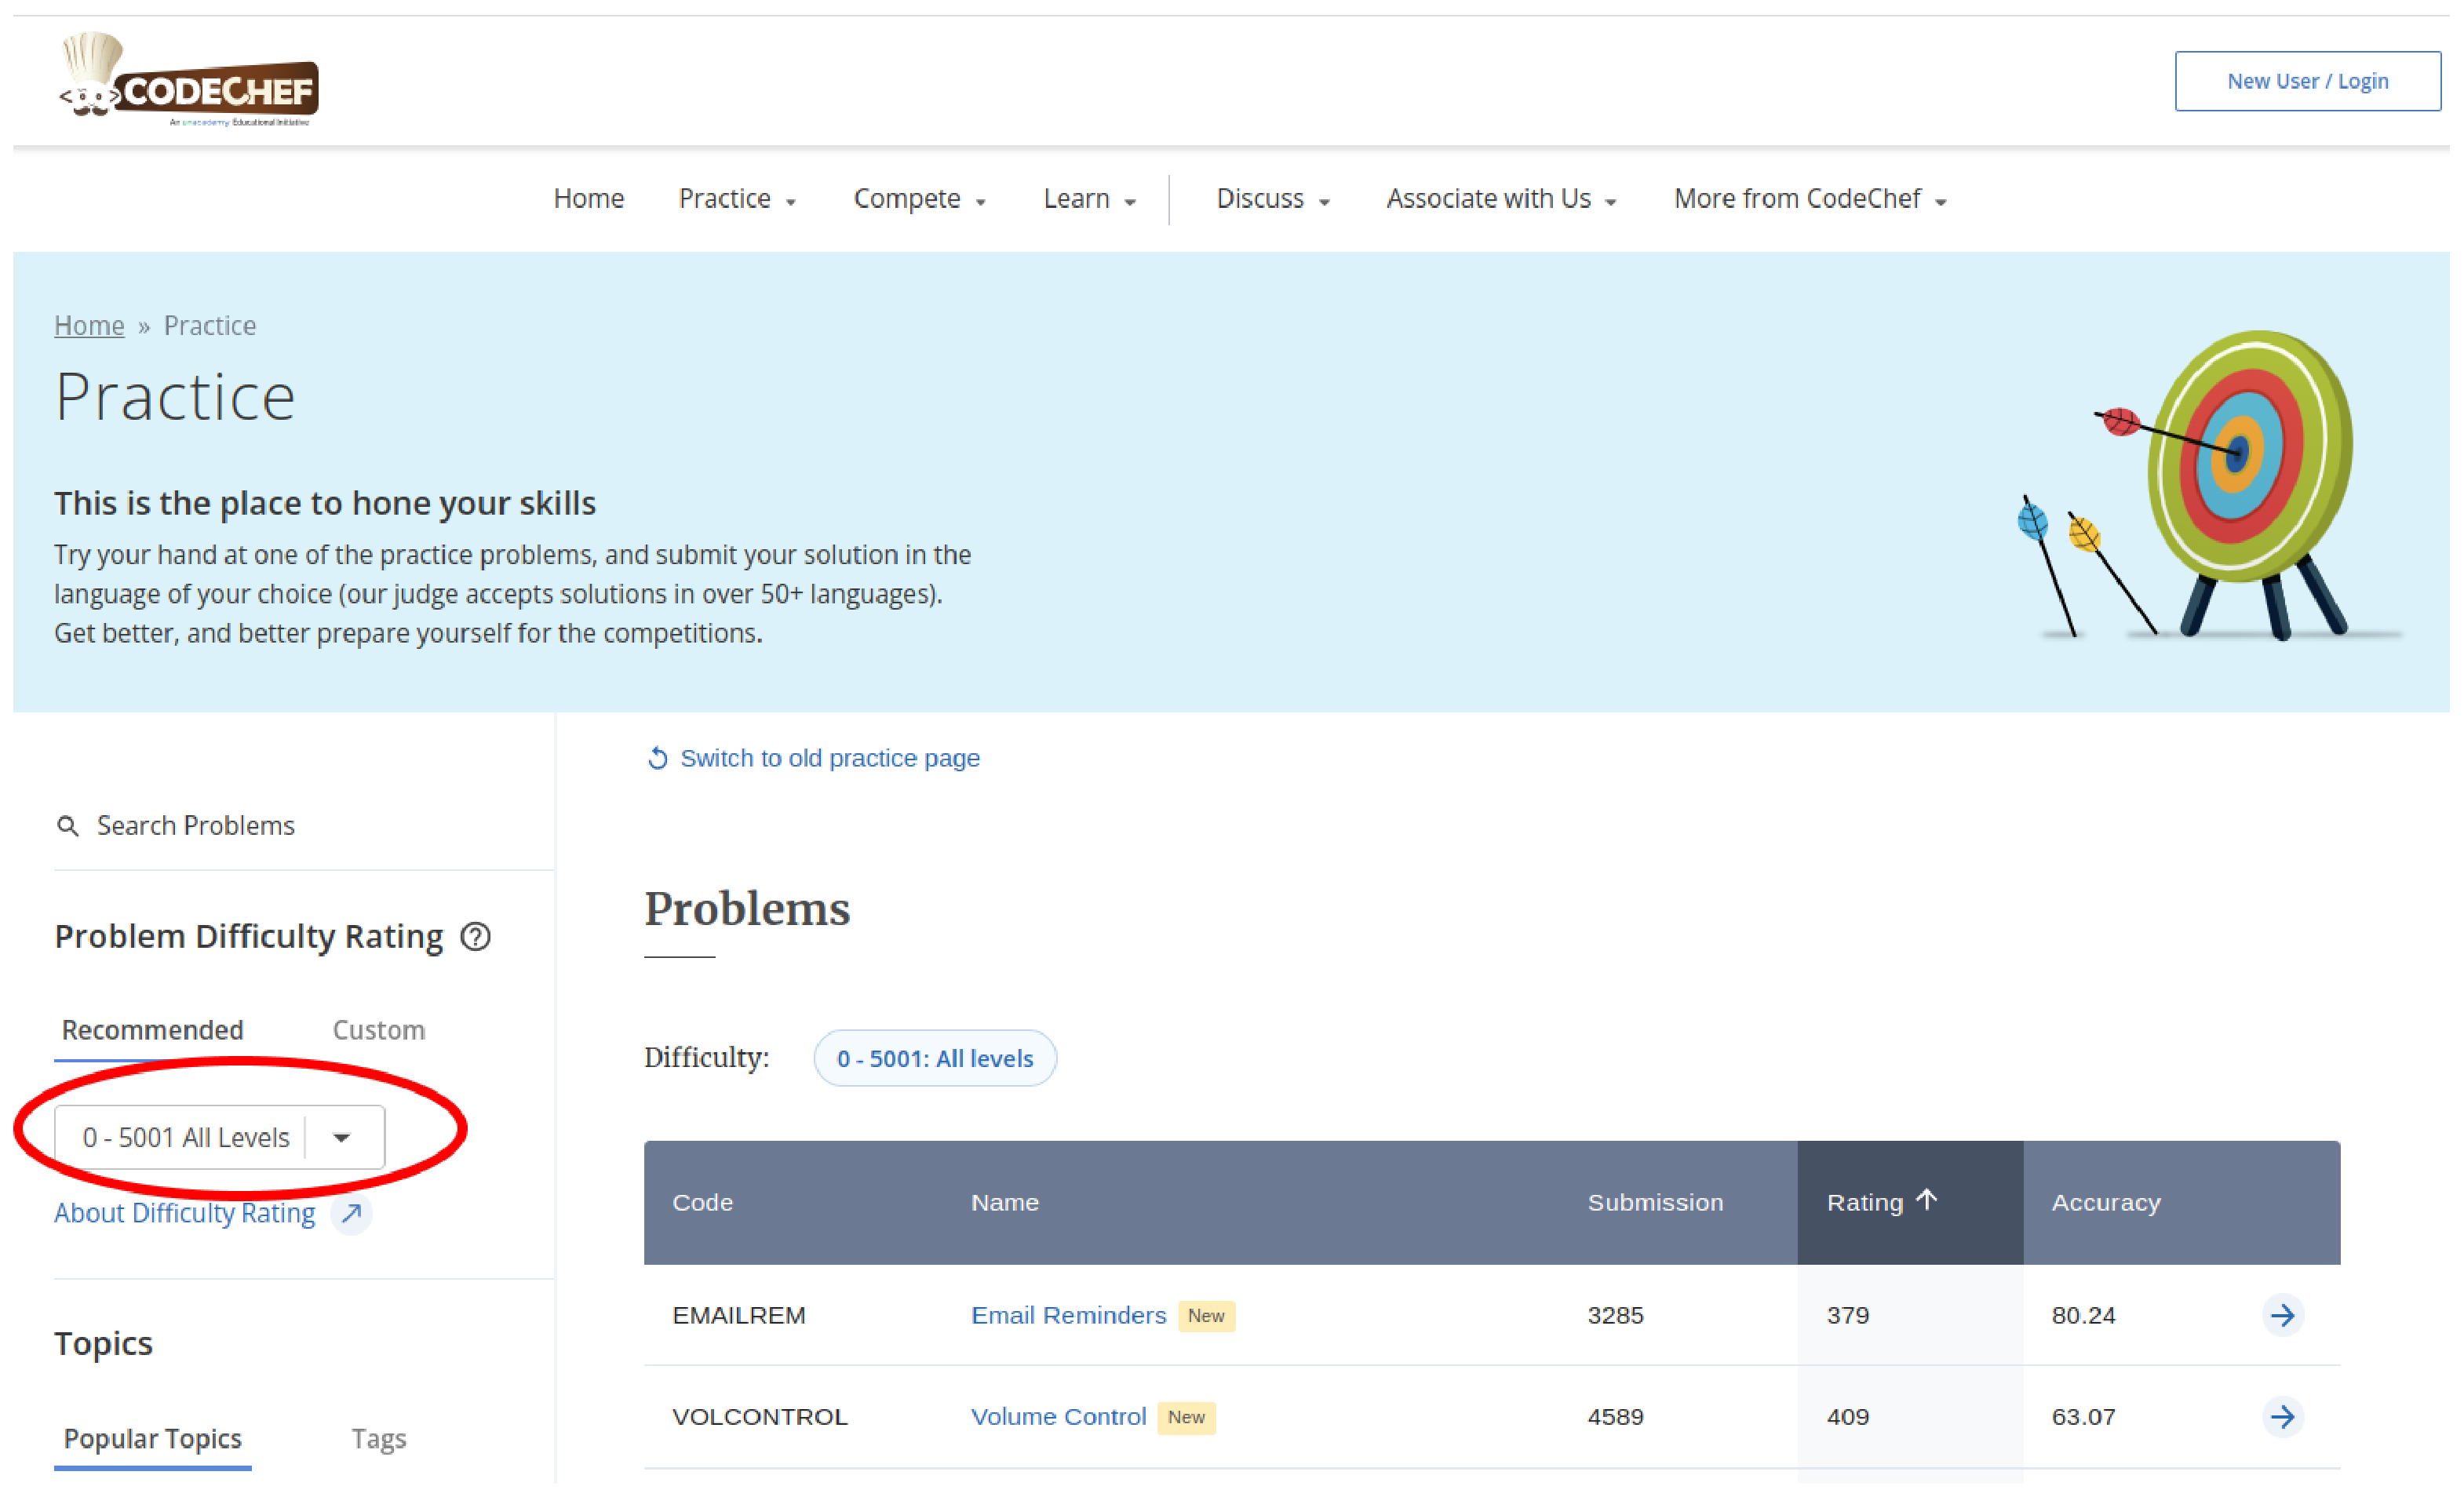
\includegraphics[keepaspectratio=true,scale=0.3]{figuras/code_chef_1.eps}
    \label{fig:code_chef_1}
    
    \medskip
    Fonte: Code Chef  (\url{https://www.codechef.com})
    \medskip
\end{figure}

\begin{figure}
    \centering
    \caption{Code Chef — Número de problemas}
    
\includegraphics[keepaspectratio=true,scale=0.3]{figuras/code_chef_2.eps}
    \label{fig:code_chef_2}
    \medskip
    Fonte: Code Chef  (\url{https://www.codechef.com})
    \medskip
\end{figure}

Para o levantamento do número de problemas no Google's Coding Competition foram separadas 3 categorias diferentes, correspondentes aos 3 eventos anuais do Google: Code Jam, KickStart e HashCode. Na categoria Code Jam existem 8 rounds diferentes, dentre eles \textit{rounds} de prática, classificatórios e os oficiais. O número de problemas das finais variam de 5 a 6 problemas, enquanto nos demais \textit{rounds} varia de 3 a 4 problemas; como até hoje foram realizadas 4 competições, começando em 2018, foi estimado um total de 120 problemas para essa categoria. Na categoria KickStart são 8 \textit{rounds} em cada edição, sendo que cada \textit{round} contém 3 problemas. A competição teve início em 2018, totalizando 4 edições, de modo que o número estimado de problemas é igual a 96. Por fim, na categoria HashCode há apenas 2 problemas por edição: 1 problema do \textit{round} classificatório e 1 do \textit{round} final, totalizando 8 problemas nas 4 edições que se iniciaram em 2018.

Não foi possível fazer o levantamento do número de problemas na plataforma CodeBench, pelo fato dos problemas serem privados. A plataforma disponibiliza para professores a criação de turma, onde o acesso é controlado, e por conta disso, não foi feita uma estimativa do número de problemas na plataforma.

Para o levantamento de problemas no Sphere Online Judge foi acessado  o menu de problemas. Nele foram localizadas 6 categorias: ``\textit{Classical}'', ``\textit{Chalenge}'', ``\textit{Partial}'', ``\textit{Tutorial}'', ``\textit{Riddle}'' e ``\textit{Basics}'', como mostra a Figura \ref{fig:spoj}. Para o levantamento do número de problemas foram acessadas cada uma das categorias, e o número de páginas por categoria foi contado. Com exceção da última página, as demais apresentam 50 problemas; portanto, para ter o total de problemas, foram contadas as páginas — exceto a última — e o resultado foi multiplicado por 50. Em seguida, foi adicionado o total de problemas da última página ao valor; na Tabela \ref{table:spoj_categories} são apresentadas as informações citadas por categoria.

\begin{figure}
    \centering
    \caption{Sphere Online Judge — Categorias de problemas}
    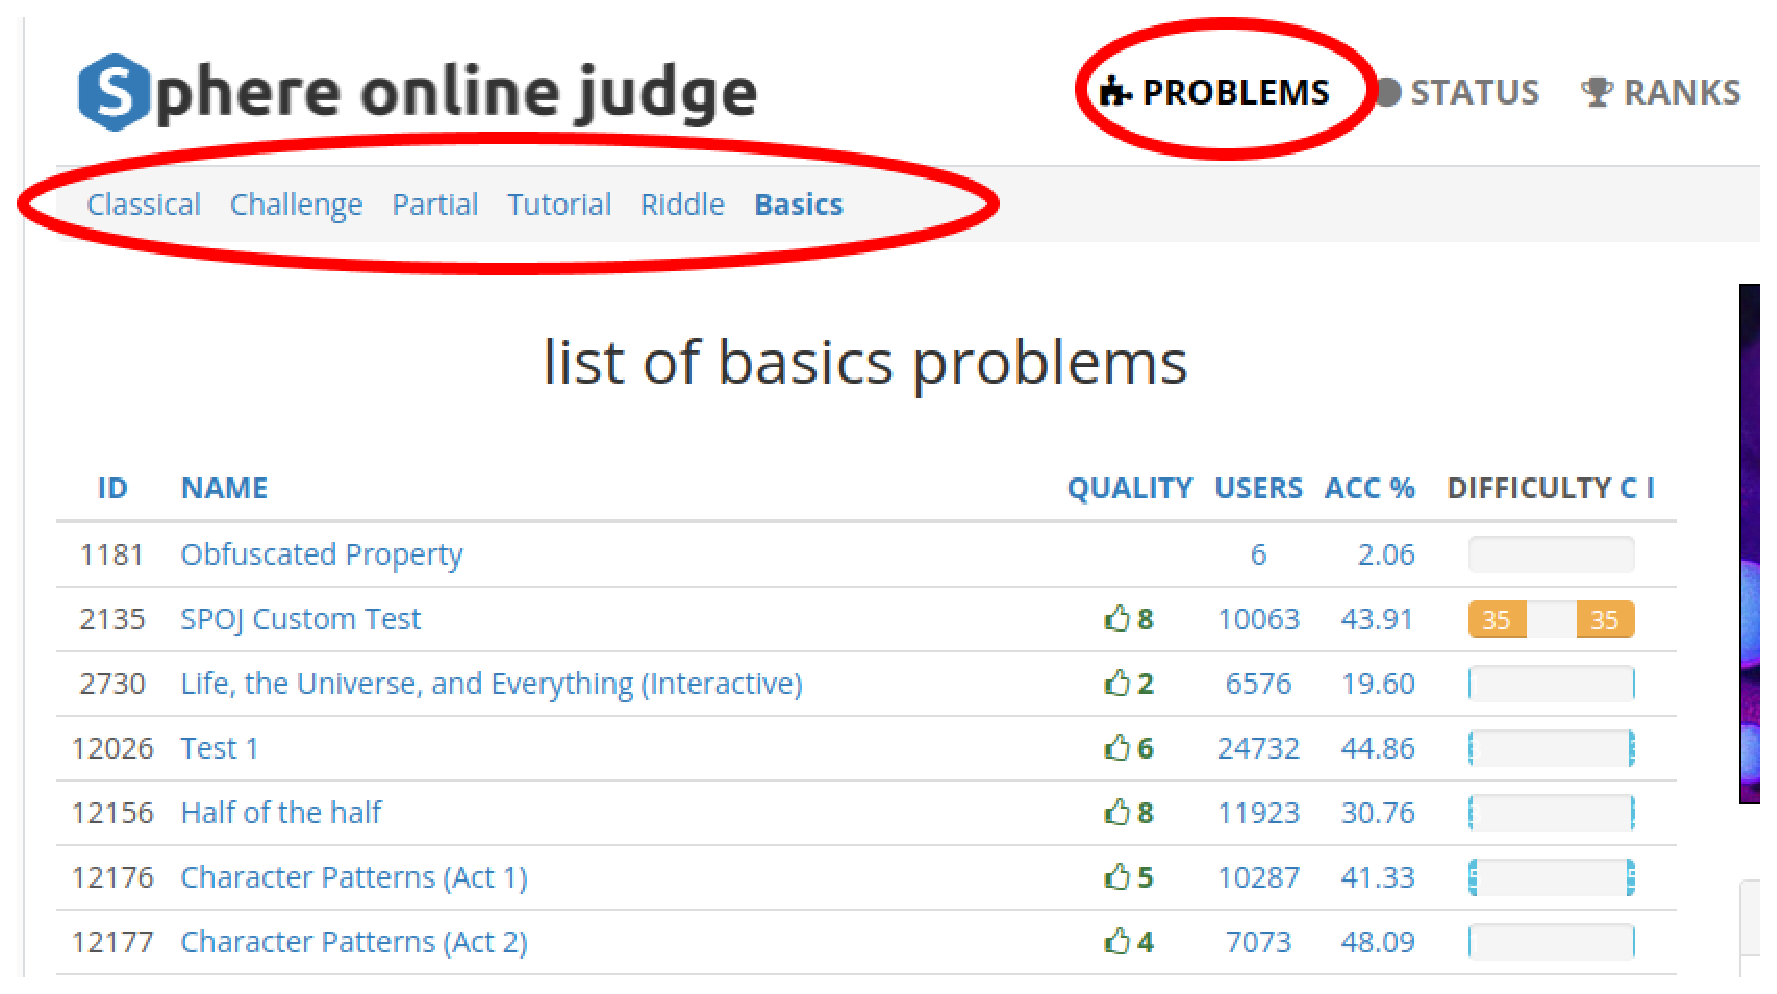
\includegraphics[keepaspectratio=true,scale=0.4]{figuras/spoj.eps}
    \label{fig:spoj}
    
    \medskip
    Fonte: Sphere Online Judge (\url{https://www.spoj.com})
    \medskip
\end{figure}

\begin{table}
    \caption[Caption for LOF]{Informações das categorias — Sphere Online Judge \footnotemark}
    \centering
    \label{table:spoj_categories}
    \begin{threeparttable}
        \begin{tabular}{lcc}
        \toprule
        \textbf{Categoria} & \textbf{Número de páginas} & \textbf{Problemas na última página} \\
        \midrule
        Classical & 79                & 50                         \\
        Chalenge  & 4                 & 10                         \\
        Tutorial  & 28                & 49                         \\
        Partial   & 1                 & 35                         \\
        Basics    & 7                 & 3    
         \\
        \bottomrule
        \end{tabular}
        \begin{tablenotes}
        \centering
        \item Fonte: Sphere Online Judge (\url{https://www.spoj.com})
        \end{tablenotes}
    \end{threeparttable}
\end{table}
\footnotetext{Data da observação: 05/04/2022}

Os demais juízes onlines possuem alguma forma de apresentar todos os problemas separados por páginas com um valor fixo de problemas em cada uma delas. Com isso, o método para contagem nos demais sites foi: o valor do número de problemas por página é multiplicado pelo total de páginas — com exceção da página final —, e depois, o número de problemas na última página é adicionado ao valor total. Na Figura \ref{fig:hackerearth_numero_problemas} é possível observar esse padrão na plataforma Hackerearth, que apresenta 77 páginas e um total de 20 problemas em cada; sem contar com a última página, é possível estimar o número de problemas em 1520.
 
\begin{figure}
    \centering
    \caption{Hackerearth — Número de problemas}
    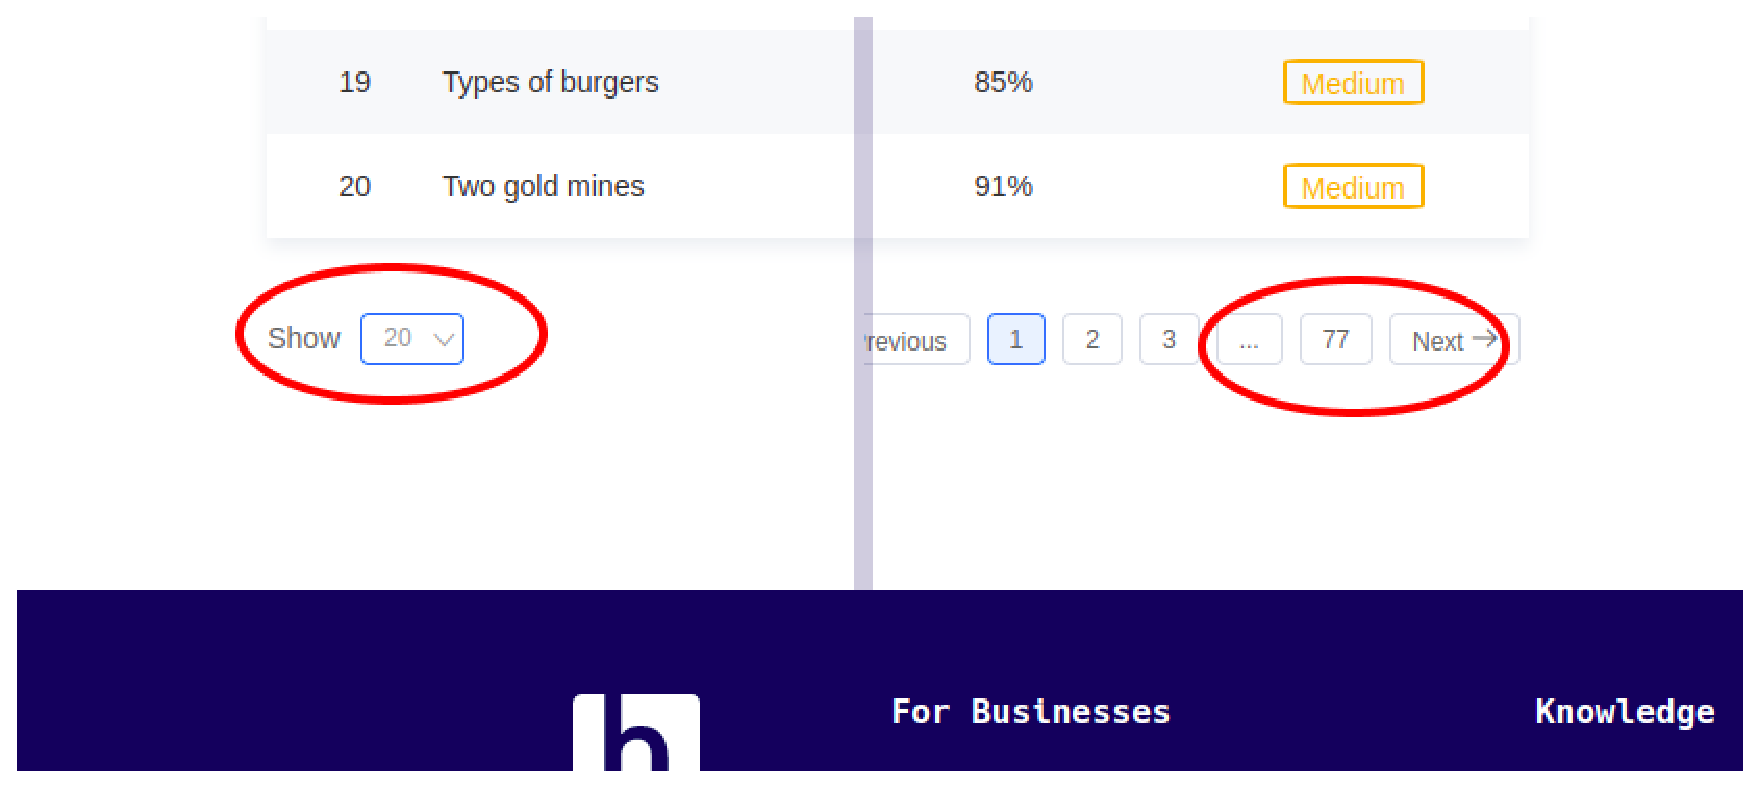
\includegraphics[keepaspectratio=true,scale=0.45]{figuras/hackerearth_numero_problemas.eps}
    \label{fig:hackerearth_numero_problemas}
    
    \medskip
    Fonte: Hackerearth (\url{https://www.hackerearth.com})
    \medskip
\end{figure}

Na Tabela \ref{table:problemas_por pagina} o levantamento dessas informações para os demais juízes é representado nas colunas: ``Problemas por página'', ``Total de páginas'' e ``Problemas na última página''; com essas informações é possível fazer uma estimativa do número total de problemas em cada uma das plataformas disponíveis na Tabela.

\begin{table}[ht]
    \caption{Coleta do número de problemas por página}
    \centering
    \label{table:problemas_por pagina}
    \begin{threeparttable}
        \begin{tabular}{lccc}
        \toprule
       \textbf{ Juíz online} &
          \begin{tabular}[c]{@{}c@{}}\textbf{Problemas} \\ \textbf{por página}\end{tabular} &
          \begin{tabular}[c]{@{}c@{}}\textbf{Total} \\ \textbf{de páginas}\end{tabular} &
          \begin{tabular}[c]{@{}c@{}}\textbf{Problemas} \\ \textbf{na última página}\end{tabular} \\
        \midrule
        Hackerearth      & 20  & 77 & 6  \\
        PKU Judge Online & 100 & 31 & 54 \\
        Neps Academy     & 16  & 67 & 13 \\
        \bottomrule
        \end{tabular}
            \begin{tablenotes}
            \centering
            \item Fonte: Hackerearth (\url{https://www.hackerearth.com})
        \end{tablenotes}
    \end{threeparttable}
\end{table}

\subsection{Levantamento das funcionalidades dos juízes}
\label{subsec:levantamento_funcionalidades}

Nessa subseção será abordada a maneira onde o levantamento das funcionalidades existentes em cada um dos juízes online foi realizada. As observações de cada um dos juízes foi efetuada de maneira diferente, apesar de a abordagem ter sido similar em aluns.

As funcionalidades do site \textit{Online Judge} foram levantadas simplesmente navegando pelo site, enviando problemas olhando a resposta e buscando por tutoriais e ferramentas adicionais no próprio site. O site possui links para ferramentas externas como \textit{uDebug}\footnote{\url{https://www.udebug.com/UVa/}}, plataforma que auxilia a solução dos problemas disponibilizado um código correto para comparação de entradas e saídas, e o \textit{uHunt} uma plataforma direcionada para o site \textit{Online Judge} que deixa a resolução de questões mais iterativa, mostrando estatísticas dos problemas resolvidos e separando as questões em categorias. 

Para o levantamento das funcionalidades no site \textit{PKU Online Judge}, foi feita uma navegação no site e acessando as funcionalidades foi possível coletar algumas informações. Ao enviar uma questão, e é possível perceber que o site aceita algumas linguagens e compiladores como mostrado na Figura \ref{fig:pku_2}, porém não foi possível receber o veredicto de uma questão enviada, pois no dia 5 de abril as 11:43, horário onde o teste foi feito, o site retornava um erro ao enviar a questão;

Já no \textit{Codeforces}, as funcionalidades foram observadas navegando e enviando questões.  O foco do site está em competições, e ocorrem competições semanalmente. Além disso, a maioria dos problemas possui tutoriais e os códigos e soluções de outras pessoas são abertos.

\section{Levantamento de requisitos}
\label{sec:levantamentoDeRequisitos}

Antes e durante o desenvolvimento do GOJ, foi necessário realizar um levantamento de requisitos. Essa etapa é importante para obter detalhadamente os recursos que englobam a aplicação \cite{young2002recommended}.

Semanalmente, foram feitas entrevistas para entendimento do GOJ, as responsabilidades do sistema e como ele deveria se comportar. Também foram feitas prototipagens para assegurar o correto andamento do desenvolvimento.

Os requisitos levantados da aplicação se dividem em três principais, descritos no Quadro \ref{table:reqGerais}:

\begin{quadro}
    \caption{Requisitos gerais}
    \centering
    \label{table:reqGerais}
    \begin{threeparttable}
    \begin{tabular}{ |p{0.5cm}|p{10cm}|  }
        \hline
        
        \textit{\textbf{Id}} & 
        \textbf{Requisito} \\
        \hline
        
        1 & É necessário armazenar questões e eventos das edições das maratonas UnB de programação, que ocorrem anualmente.  \\
        \hline
        
        2 & O usuário deve conseguir enviar sua solução em código para ela ser julgada, retornando um veredicto de sua submissão.  \\ 
        \hline
        
        3 & O usuário deve conseguir ter acesso aos problemas e eventos.  \\
        \hline
    \end{tabular}
    \medskip
    \begin{tablenotes}
        \centering
        \item Fonte: o Autor
    \end{tablenotes}
    \end{threeparttable}

\end{quadro}

Os requisitos citados no Quadro \ref{table:reqGerais} são requisitos amplos e com pouca especificidade. Para não gerar ambiguidade ou incompletude para os mesmos, eles foram divididos em requisitos menores e mais específicos. Com isso, mais detalhes foram listados na busca de uma maior completude e clareza. Os requisitos menores serão descritos nas seguintes subseções: \nameref{subsec:storage}, \nameref{subsec:juiz} e \nameref{subsec:ui}.

\subsection{Armazenamento das questões e eventos}
\label{subsec:storage}

As informações dos eventos e questões das maratonas UnB de programação precisam ser armazenadas e disponibilizadas para o funcionamento do GOJ; os requisitos dessa Subseção são sobre o armazenamento dessas informações. No Quadro \ref{table:reqArmazenamento} são mostrados os requisitos referentes ao armazenamento de questões e eventos do GOJ.

\begin{quadro}
    \caption{Requisitos de armazenamento}
    \centering
    \label{table:reqArmazenamento}
    \begin{threeparttable}
    \begin{tabular}{ |p{0.6cm}|p{10cm}|  }
        \hline
        
        \textbf{Id} & 
        \textbf{Requisito} \\
        \hline
        
        1.1 & As questões devem possuir título, enunciado, tempo limite de execução, limite de memória utilizado pelo programa, lista de rótulos que categorizam o problema, ID predefinido para localização e identificação das questões. \\
        \hline
        
        1.2 & As questões possuem arquivos, utilizados para julgar as submissões enviadas.\footnotemark 
        \\
        \hline
        
        1.3 & Os eventos devem possuir uma data, que identifica quando o evento aconteceu, um nome e uma lista de problemas, tal como o rótulo do problema naquele evento, ex: ``Questão A''.  \\ 
        \hline
        
        1.4 & Além das informações dos problemas, as soluções e lista de testes precisam ser armazenadas.  \\
        \hline
    \end{tabular}
    \medskip
    \begin{tablenotes}
        \centering
        \item Fonte: o Autor
    \end{tablenotes}
    \end{threeparttable}
    
\end{quadro}
\footnotetext{Os arquivos necessários de cada questão dependem da questão e do juiz eletrônico utilizado para julgar as submissões enviadas}

Os requisitos citados no Quadro \ref{table:reqArmazenamento} tem uma granularidade maior que os citados no Quadro \ref{table:reqGerais}. Com isso, o desenvolvimento das funcionalidades se torna mais preciso, evitando que expressões genéricas gerem ambiguidades com as necessidades da aplicação.

\subsection{Juiz eletrônico}
\label{subsec:juiz}

Quando o usuário escreve um código com sua solução para algum problema, o código deve ser julgado e o usuário deve conseguir ver o veredito de sua submissão. Para isso o GOJ precisa de um juiz eletrônico. No Quadro \ref{table:reqJuiz}, estão listados requisitos específicos para o juiz eletrônico do GOJ

\begin{quadro}
    \caption{Requisitos do juiz}
    \centering
    \label{table:reqJuiz}
    \begin{threeparttable}
    \begin{tabular}{ |p{0.6cm}|p{11cm}|  }
        \hline
        
        \textbf{Id} & 
        \textbf{Requisito} \\
        \hline
        
        2.1 & 
        O sistema deve receber arquivos ou textos contendo códigos em linguagens de programação pré, definidas. \\ 
        \hline
        
        2.2 & 
        As linguagens suportadas pelo sistema devem ser as mesmas linguagens utilizadas no ICPC. \\
        \hline
        
        2.4 & 
        O sistema deve conseguir saber a memória e tempo utilizados para execução do programa. \\
        \hline
    \end{tabular}
    \medskip
    \begin{tablenotes}
        \centering
        \item Fonte: o Autor
    \end{tablenotes}
    \end{threeparttable}
    
\end{quadro}

Os requisitos citados no Quadro \ref{table:reqJuiz} se relacionam com a parte do GOJ que julgará os códigos enviados pelos usuários. Os requisitos citados estão relacionados com os formatos das questões do GOJ. Por seguir o padrão de maratona ICPC, o juiz eletrônico do GOJ deve ter um suporte similar.

%% TODO parei aqui
\subsection{Interface de usuário}
\label{subsec:ui}

A interface de usuário é responsável por apresentar as informações do GOJ ao usuário e proporcionar mecanismos de iteração do usuário com a aplicação. Os requisitos listados no Quadro \ref{table:reqInterface} são referentes a interface de usuário do GOJ, são requisitos referentes as informações das questões que serão disponibilizadas ao usuário.

\begin{quadro}
    \caption{Requisitos da interface}
    \centering
    \label{table:reqInterface}
    \begin{threeparttable}
    \begin{tabular}{ |p{0.6cm}|p{10cm}|  }
        \hline
        
        \textbf{Id} & 
        \textbf{Requisito} \\
        \hline
        
        3.1 & 
        As informações das questões devem estar disponíveis ao usuário, podendo conter formulas matemáticas e imagens. \\
        \hline
        
        3.2 & 
        Os eventos devem ser apresentados ao usuário de maneira organizada, com a lista dos respectivos problemas dos eventos.  \\ 
        \hline
        
        3.3 & 
        As informações de dicas e tutoriais das questões dever ser escondidas do usuário e disponíveis apenas se o usuário optar por elas.  \\
        \hline
    \end{tabular}
        \medskip
    \begin{tablenotes}
        \centering
        \item Fonte: o Autor
    \end{tablenotes}
    \end{threeparttable}

\end{quadro}

Os requisitos no Quadro \ref{table:reqInterface} descrevem como a interface deve ser. Ela se assemelha a juízes onlines presentes hoje, porém um foco direcionado para essa interface é ser amigável para estudantes iniciantes em programação, e ser compatível com os elementos não textuais necessários para as questões das maratonas UnB de programação.

\section{Arquitetura}
\label{sec:arquitetura}

A arquitetura escolhida para construção do GOJ foi a de micro-serviços, separando a aplicação em módulos com pequenos conjuntos de responsabilidades individuais. Além dos módulos desenvolvidos, foram utilizados os seguintes servições externos: serviço de filas, de notificações e de armazenamento. A Figura \ref{fig:arquitetura_goj} representa a arquitetura do Gamma Online Judge e os módulos desenvolvidos: ``Gamma Judge Admin'', ``Gamma Judge UI'', ``Gamma Judge API'' e ``Gamma Judge Tools''.

\begin{figure}
    \centering
    \caption{Arquitetura geral GOJ}
    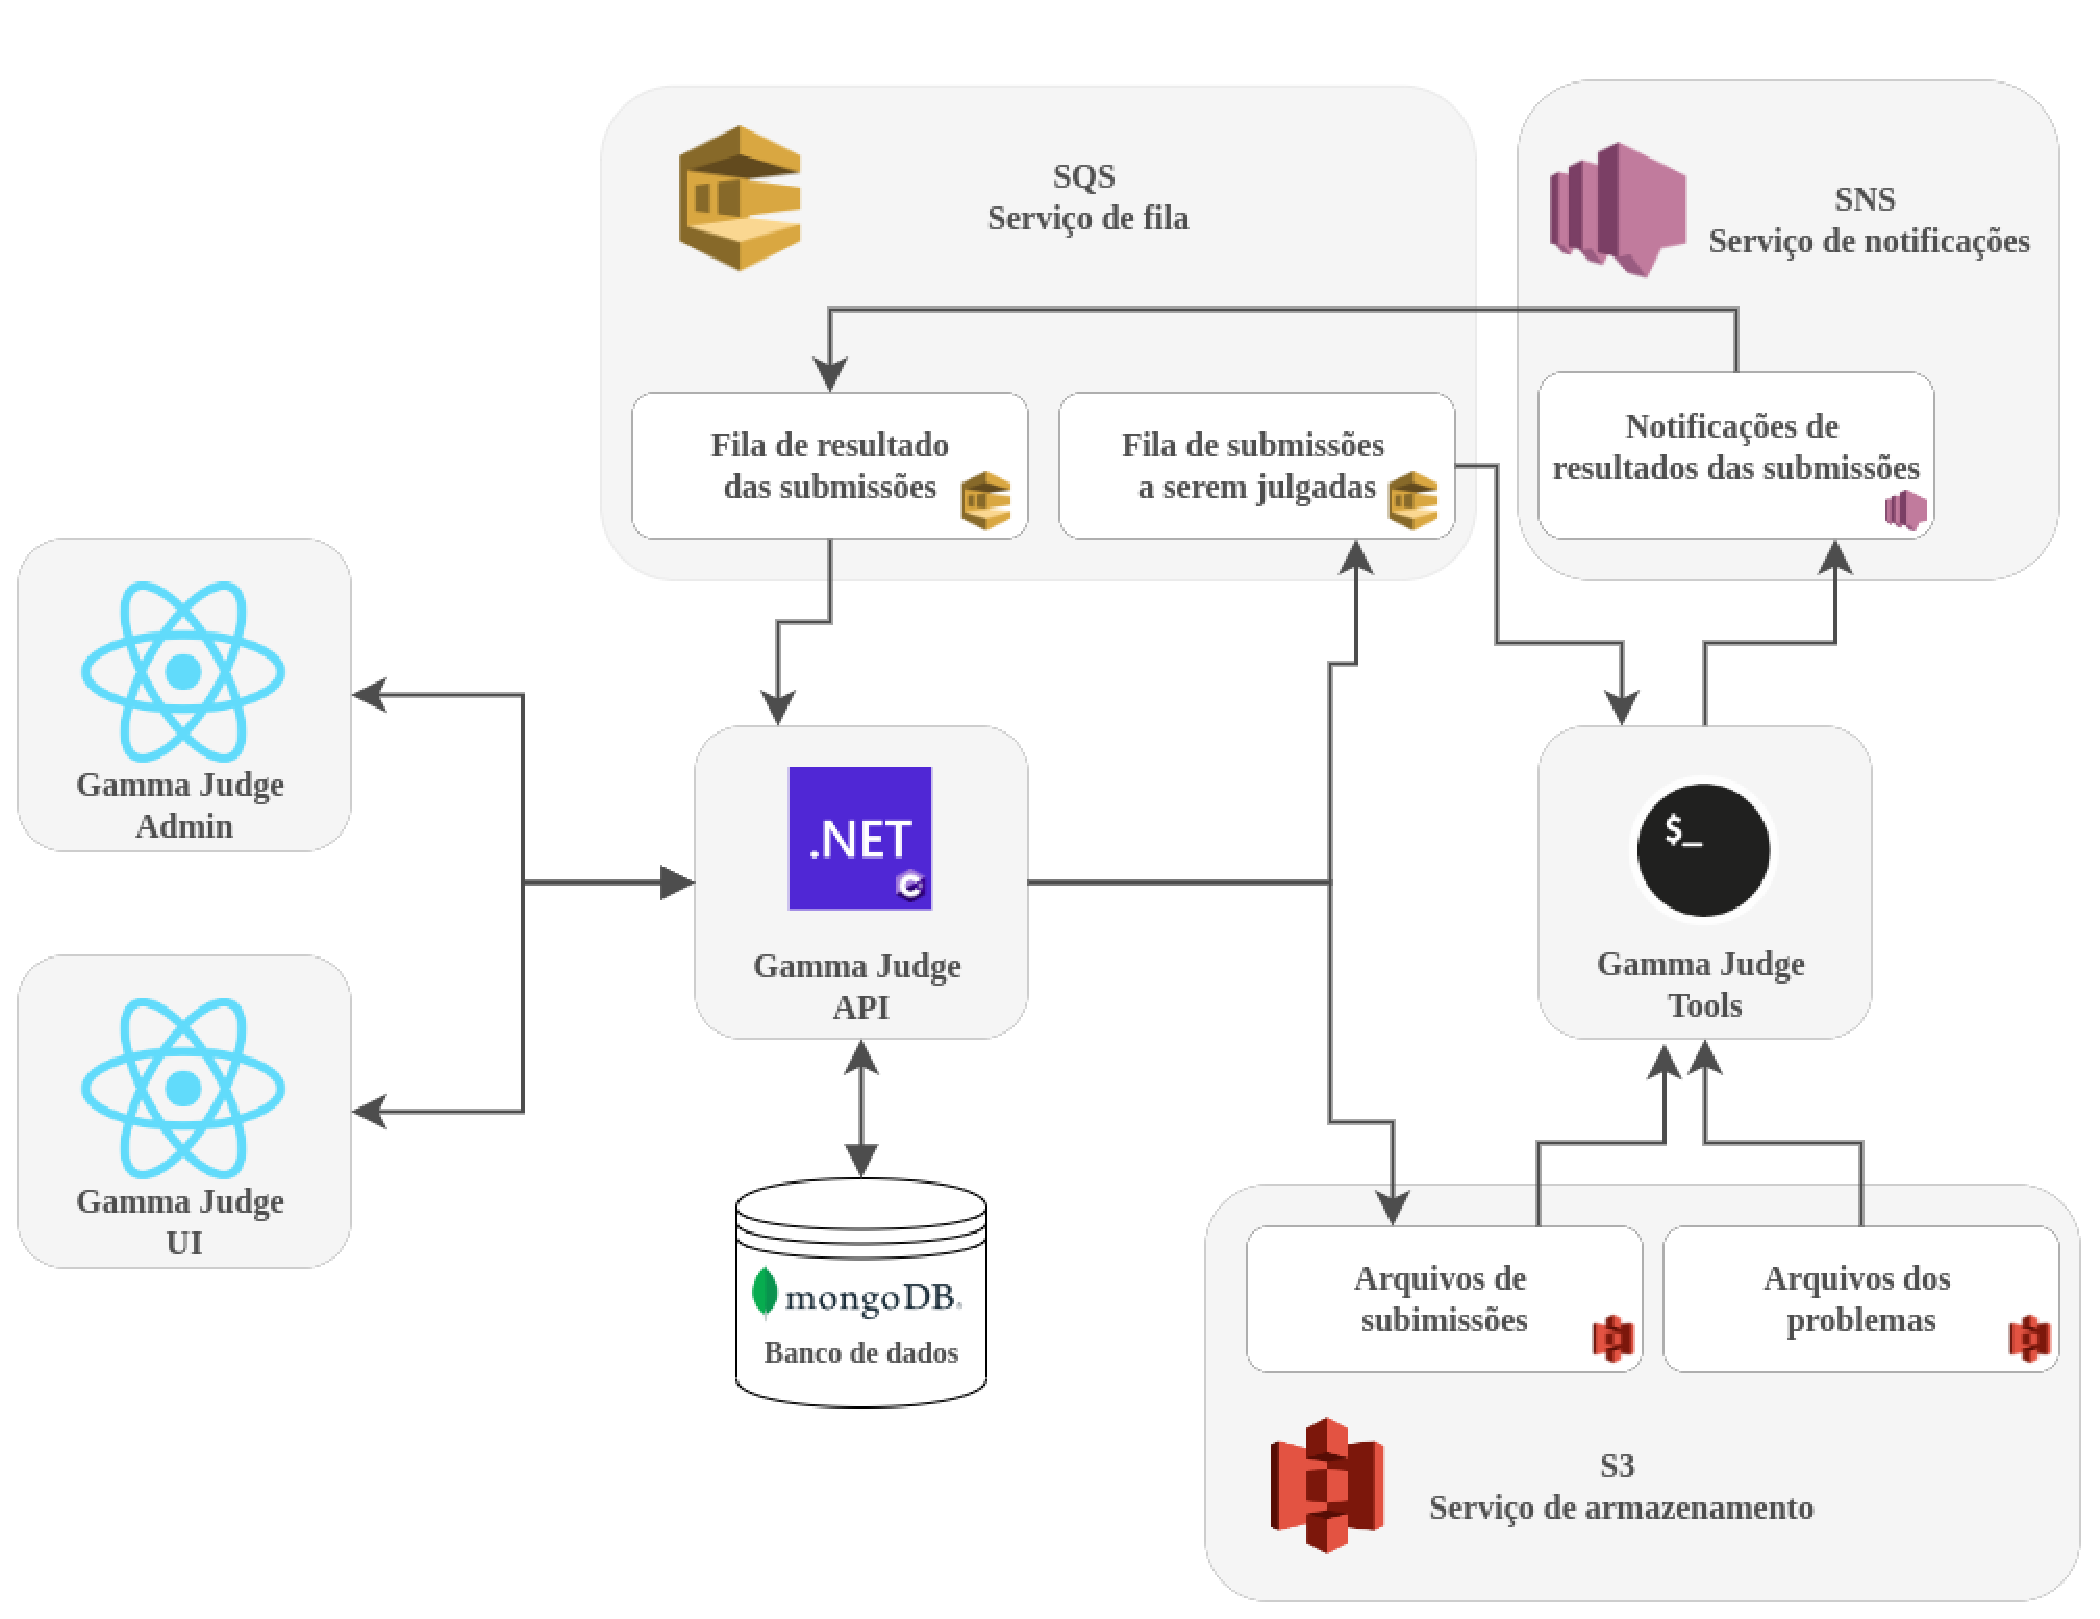
\includegraphics[keepaspectratio=true,scale=0.45]{figuras/arquitetura_goj.eps}
    \label{fig:arquitetura_goj}
    \medskip
    Fonte: o Autor
    \medskip
\end{figure}

Nessa seção serão abordadas as arquiteturas, tecnologias e os métodos utilizados para o desenvolvimento dos módulos. Também serão abordadas as ferramentas e serviços externos utilizados no desenvolvimento do GOJ.

\subsection{Servições externos} 
\label{subsec:arquitetura_servicos_ext}

Na arquitetura proposta, foram utilizados recursos do AWS Console\footnote{\url{https://aws.amazon.com/pt/console/}}, o qual disponibiliza ferramentas diversas para a manutenção, processamento e armazenamento de aplicações na nuvem; além disso, existem serviços prontos que auxiliam o desenvolvimento de aplicações. No GOJ, os serviços AWS que fazem parte da arquitetura são: Simple Queue Service (SQS), o Simple Notification Service (SNS) e o Simple Storage Service (S3).

O SQS consiste em um serviço online de filas, onde mensagens podem ser enviadas, lidas e consumidas. A ideia da utilização desse serviço é manter a consistência do funcionamento da aplicação em casos de intermitência ou erros do sistema. No GOJ, o serviço SQS é utilizado para que a comunicação entre o módulo Gamma Judge API — que recebe as submissões do usuário — e o módulo Gamma Judge Tools — que julga as submissões lidas da fila — seja consistente. No caso do Gamma Online Judge apresentar falhas pontuais para julgar as submissões — como falta de memória na máquina, inatividade do serviço, etc. — a mensagem não será consumida ou ficará no sistema de filas até isso acontecer; esta abordagem resulta em maior consistência, pois, em caso de inatividade ou intermitência do Gamma Judge Tools, o envio de submissões não será comprometido.

Já o SNS é um serviço de notificações, que permite que uma mensagem enviada possa ser distribuída para outros serviços. Sua utilização no GOJ consiste em notificar quando uma submissão for julgada, sendo esta notificação enviada através de um tópico SNS e os serviços inscritos nesse tópico recebem a mensagem. A ``Fila de resultados das submissões'' é inscrita no tópico SNS ``Notificações de resultados das submissões'', como apresentado na Figura \ref{fig:arquitetura_goj}, e todas as mensagens enviadas nesse tópico são enviadas para a fila, para que os resultados possam ser consumidos e apresentados ao usuário final.

Por fim, o S3 é um serviço de armazenamento de arquivos. Ele é utilizado para ler e armazenar os arquivos enviados nas submissões e os arquivos necessários para julgar os problemas. A utilização de um serviço de armazenamento permite que os arquivos sejam acessados por mais de um módulo da aplicação, como acontece na arquitetura do GOJ.

\subsection{Gamma Judge API} 
\label{subsec:arquitetura_judge_api}

O módulo Gamma Judge API é responsável por fazer uma ponte de comunicação com a interface, disponibilizando as informações armazenadas e recebendo arquivos para serem julgados pelo juiz eletrônico. Além disso, é responsabilidade desse módulo processar as informações dos resultados das submissões. Na Figura \ref{fig:arquitetura_goj_api} são apresentados os fluxos descritos e as interações com a interface e os serviços externos.

\begin{figure}
    \centering
    \caption{Arquitetura — Gamma Judge API}
    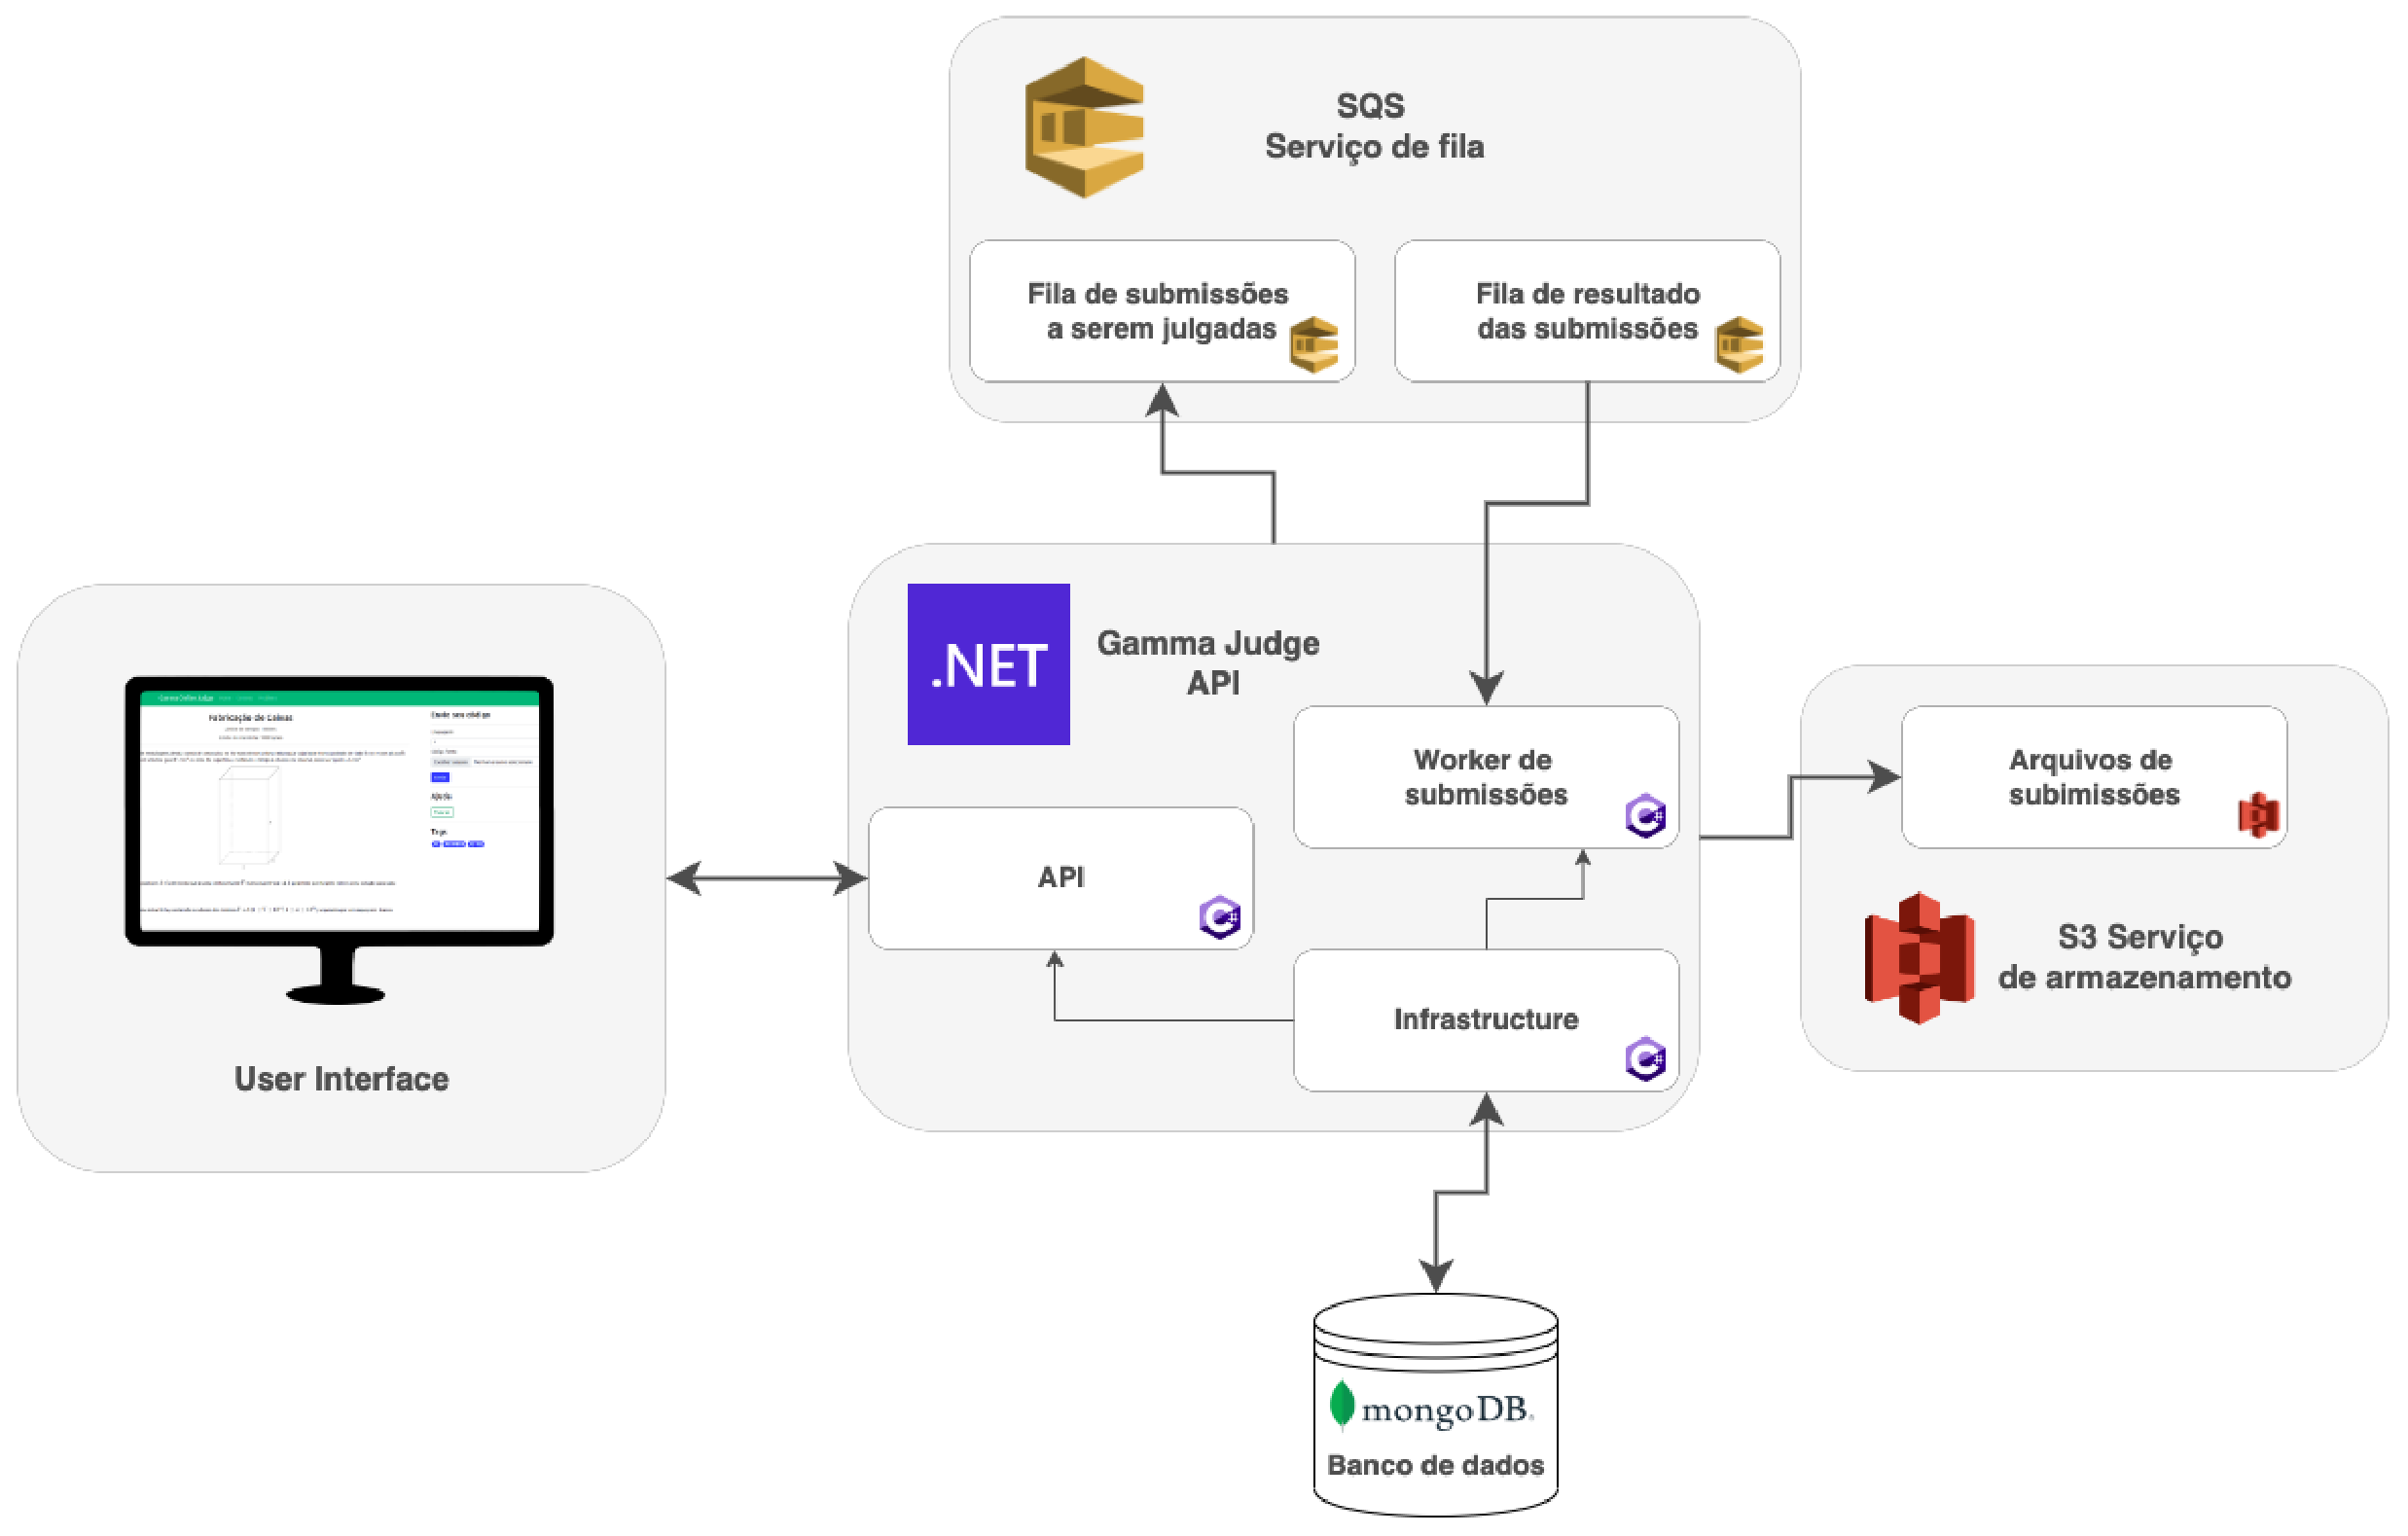
\includegraphics[keepaspectratio=true,scale=0.35]{figuras/arquitetura_goj_api.eps}
    \label{fig:arquitetura_goj_api}
    \medskip
    Fonte: o Autor
    \medskip
\end{figure}

Conforme dito anteriormente, o sistema faz o uso de 2 serviços externos: SQS e S3. O SQS é utilizado para receber as informações dos resultados das submissões e para o envio de submissões a serem julgadas. Já o serviço S3 é utilizado para o armazenamento dos arquivos de submissões. 

O Gamma Judge API se divide em 3 grandes partes: ``API'', ``Worker de submissões'' e ``Infrastructure'', como mostra a Figura \ref{fig:arquitetura_goj_api}. A ``API'' é responsável pela comunicação externa, recebendo e enviando informações para uma interface de usuário; o ``Worker de submissões'' é um \textit{background service} que processa as submissões recebidas; e a ``Infrastructure'' é uma abstração dos serviços externos, que se comunica diretamente com o banco de dados e os serviços SQS e S3, disponibilizando funções para os demais módulos.

Para o envio de uma submissão, a API recebe um arquivo, que contém a solução proposta pelo usuário, as configurações (como linguagem e compilador que serão utilizados) e as informações do problema, as quais determinarão quais são as entradas e saídas esperadas. Após recebidas, as informações da submissão são armazenadas no banco de dados, o código-fonte é enviado para o S3 com um identificador único, que associa aquele arquivo 
à submissão, e as informações são enviadas para a ``Fila de submissões a serem julgadas'' no SQS; posteriormente um juiz eletrônico é responsável por reunir esses dados e julgar o problema. Após julgada, o resultado da submissão é enviado para a fila SQS ``Fila de resultado das submissões'', onde os resultados são processados e atualizados no banco de dados.

Esse módulo foi desenvolvido utilizando o .NET Frameweork com C\# de linguagem de programação principal. O banco de dados é um MongoDB, para o armazenamento das informações de questões, eventos e submissões. A comunicação com a ``User interface'' é feita via protocolo HTTP, para o recebimento e disponibilização de informações (veja a Seção \ref{sec:apis}). Para melhora da compatibilidade e facilidade com a entrega desse sistema foi utilizada a ferramenta Docker, um sistema de virtualização que permite que o projeto seja executado em qualquer plataforma que suporte a ferramenta.

\subsection{Gamma Judge Tools} 
\label{subsec:arquitetura_judge_tools}

O Gamma Judge Tools é o módulo responsável por julgar submissões e retornar o veredicto. Esse módulo realiza o papel de um juiz eletrônico e funciona com o auxílio dos serviços externos citados na Subseção \ref{subsec:arquitetura_servicos_ext}. Os serviços externos utilizados nesse módulo são: SQS, SNS e S3, como mostra a Figura \ref{fig:arquitetura_goj_tools}.

\begin{figure}
    \centering
    \caption{Arquitetura — Gamma Judge Tools}
    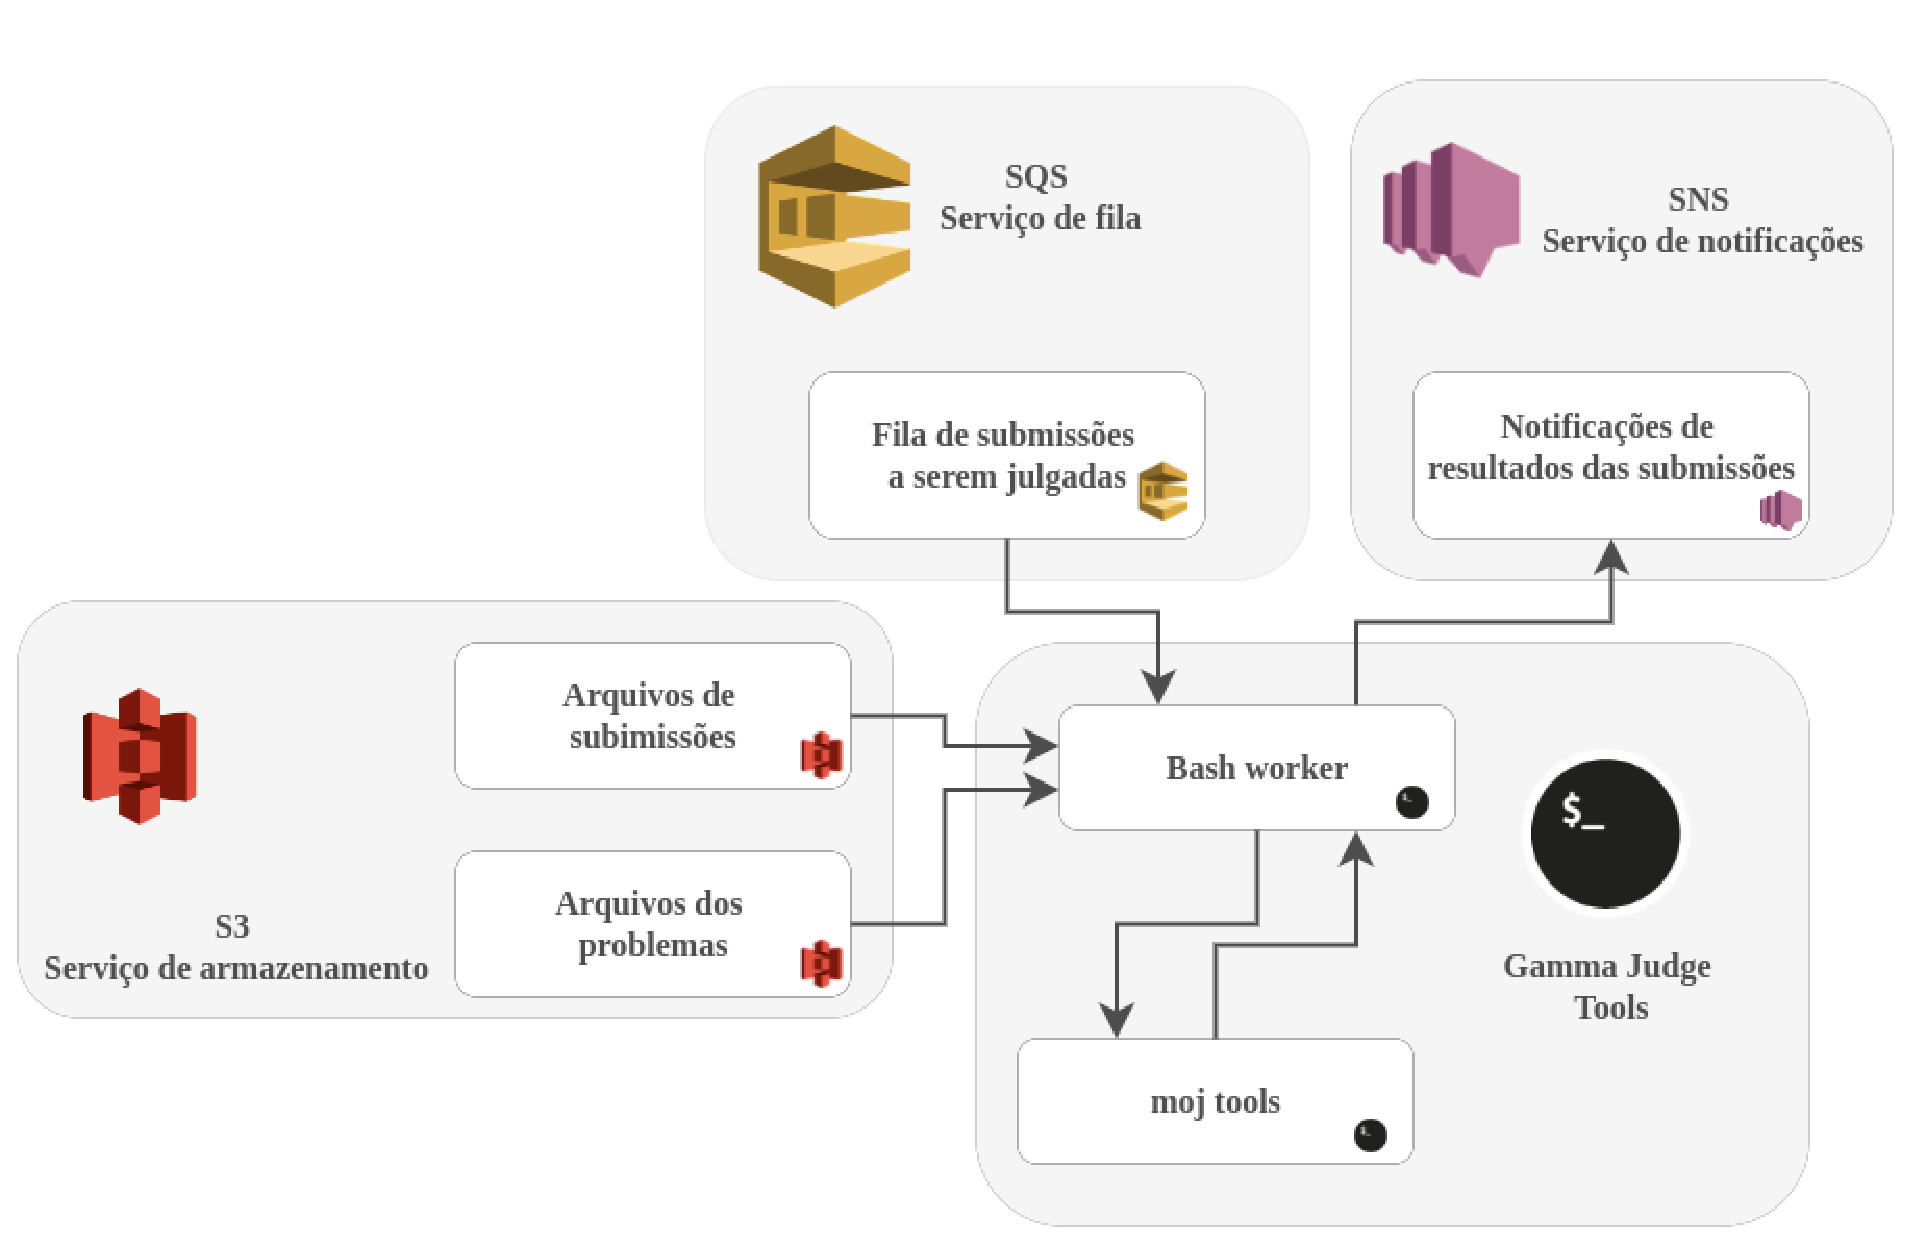
\includegraphics[keepaspectratio=true,scale=0.45]{figuras/arquitetura_goj_tools.eps}
    \label{fig:arquitetura_goj_tools}
    \medskip
    Fonte: o Autor
    \medskip
\end{figure}

O módulo foi desenvolvido em linguagem de programação Bash e possui um \textit{worker} para consumir as submissões. Cada submissão recebida possui as informações do problema correspondente: linguagem, identificador do problema e o identificador do arquivo armazenado no S3. Reunidas as informações, o módulo vai produzir, a partir do código-fonte, um código executável. Este executável será alimentado com várias entradas que correspondem aos testes do problema, e para cada entrada ele produzirá uma saída correspondente, denominada resposta. A resposta para cada entrada será confrontada com as respostas esperadas, armazenadas no S3. A comparação entre estas respostas e o comportamento do executável serão avaliados de modo a produzir um veredito para a submissão; o veredito da execução é enviado para uma notificação SNS, podendo ser: AC, WA, TLE, MLE ou RTE (veja a Seção \ref{sec:juizesOnline}). Em caso de falha do juiz na execução, a mensagem não é consumida e volta para a fila SQS para ser processada novamente.

Por esse módulo ser um serviço separado do Gamma Judge API, não é necessária sua exposição à \textit{web}. Além disso, as filas SQS realizam o controle de concorrência caso mais de um consumidor esteja acessando esse recurso, possibilitando um escalonamento do sistema, ou seja, caso seja necessário mais processamento ou paralelismo para julgar as questões, basta rodar o Gamma Judge Tools em uma máquina adicional, sem se preocupar com a concorrência entre os consumidores e a fila SQS. 

\subsection{Gamma Judge UI e Gamma Judge Admin} 
\label{subsec:arquitetura_judge_ui}

O Gamma Judge UI é a interface de usuário que se comunica com a API, recebendo e enviando informações. Ela recebe as informações dos problemas, eventos e submissões, e envia os códigos para serem processados. O Gamma Judge Admin tem um comportamento similar, porém as informações enviadas são para edição, criação e exclusão de problemas e eventos. 

Ambos os módulos foram desenvolvidos em Node JS, com Typescript sendo a linguagem principal. Nos módulos foram utilizados \textit{Node Packages}, bibliotecas externas que facilitam o desenvolvimento web (veja a Seção \ref{sec:desenvolvimentoWEB}). Das bibliotecas utilizadas, as principais foram: \textit{React Bootstrap}\footnote{https://react-bootstrap.github.io/}, que disponibiliza componentes, como botões, textos e tabelas; \textit{React Router}\footnote{https://v5.reactrouter.com/web/guides/quick-start}, que disponibiliza recursos para navegação; e \textit{React \LaTeX}\footnote{https://www.npmjs.com/package/react-latex}, que permite a renderização de elementos HTML e \LaTeX.

O Gamma Judge UI é responsável por renderizar elementos não textuais, como fórmulas, imagens e elementos necessários para a visualização das informações de um problema. As informações são recebidas em texto (texto bruto, HTML ou \LaTeX) da API, e o sistema é responsável por transformar essas informações em elementos visuais como fórmulas, tabelas ou imagens. Para isso, o pacote \textit{React \LaTeX} é utilizado, pois, permite a inserção de trechos em \LaTeX ou HTML para a visualização na página WEB.


